\chapter{实体-联系模型}

\begin{introduction}[期末考试提纲]
    \item 实体、联系、属性
    \item 超码、候选码、主码
    \item 联系的种类、联系的势
    \item 弱实体、特化、概化、聚集
    \item E-R图概念模型设计应用实例
    \item E-R图和关系模式的相互转换
\end{introduction}

\section{E-R模型基本概念}

E-R模型: Entity-Relation Model.
\begin{itemize}
    \item 世界是由一组称为实体的基本对象和这些对象之间的联系构成的.
    \item \textcolor{red}{实体(Entity)}: \textcolor{red}{客观存在}并\textcolor{red}{可相互区分}的事物叫实体.
    \item 属性(Attribute): 实体具有的某一特性称为属性. 用椭圆表示.
    \item 域(Domain): 属性的取值范围称为域.
    \item 实体型(Entity Type): 实体名+属性名集合. e.g. 学生(学号, 姓名, 年龄, 性别, 系, 年级)
    \item 实体集(Entity Set): 同类型的实体的集合. 用矩形表示.
    \item 联系(Relationship): 实体之间的相互关联. 联系也可以有属性. 用联系表示.
    \item 联系的元(Degree): 参与联系的实体集的个数.
    \begin{itemize}
        \item 学生与学生的班长联系: 一元. 只有一个实体集.
        \item 有时称一元联系为递归联系.
        \item 联系是发生在实体集之间的还是实体型之间的? \textbf{实体集.}
    \end{itemize}
    \item 实体集属性中作为主码的一部分的属性用\underline{下划线}来标明.
\end{itemize}

\begin{figure}[H]
    \centering
    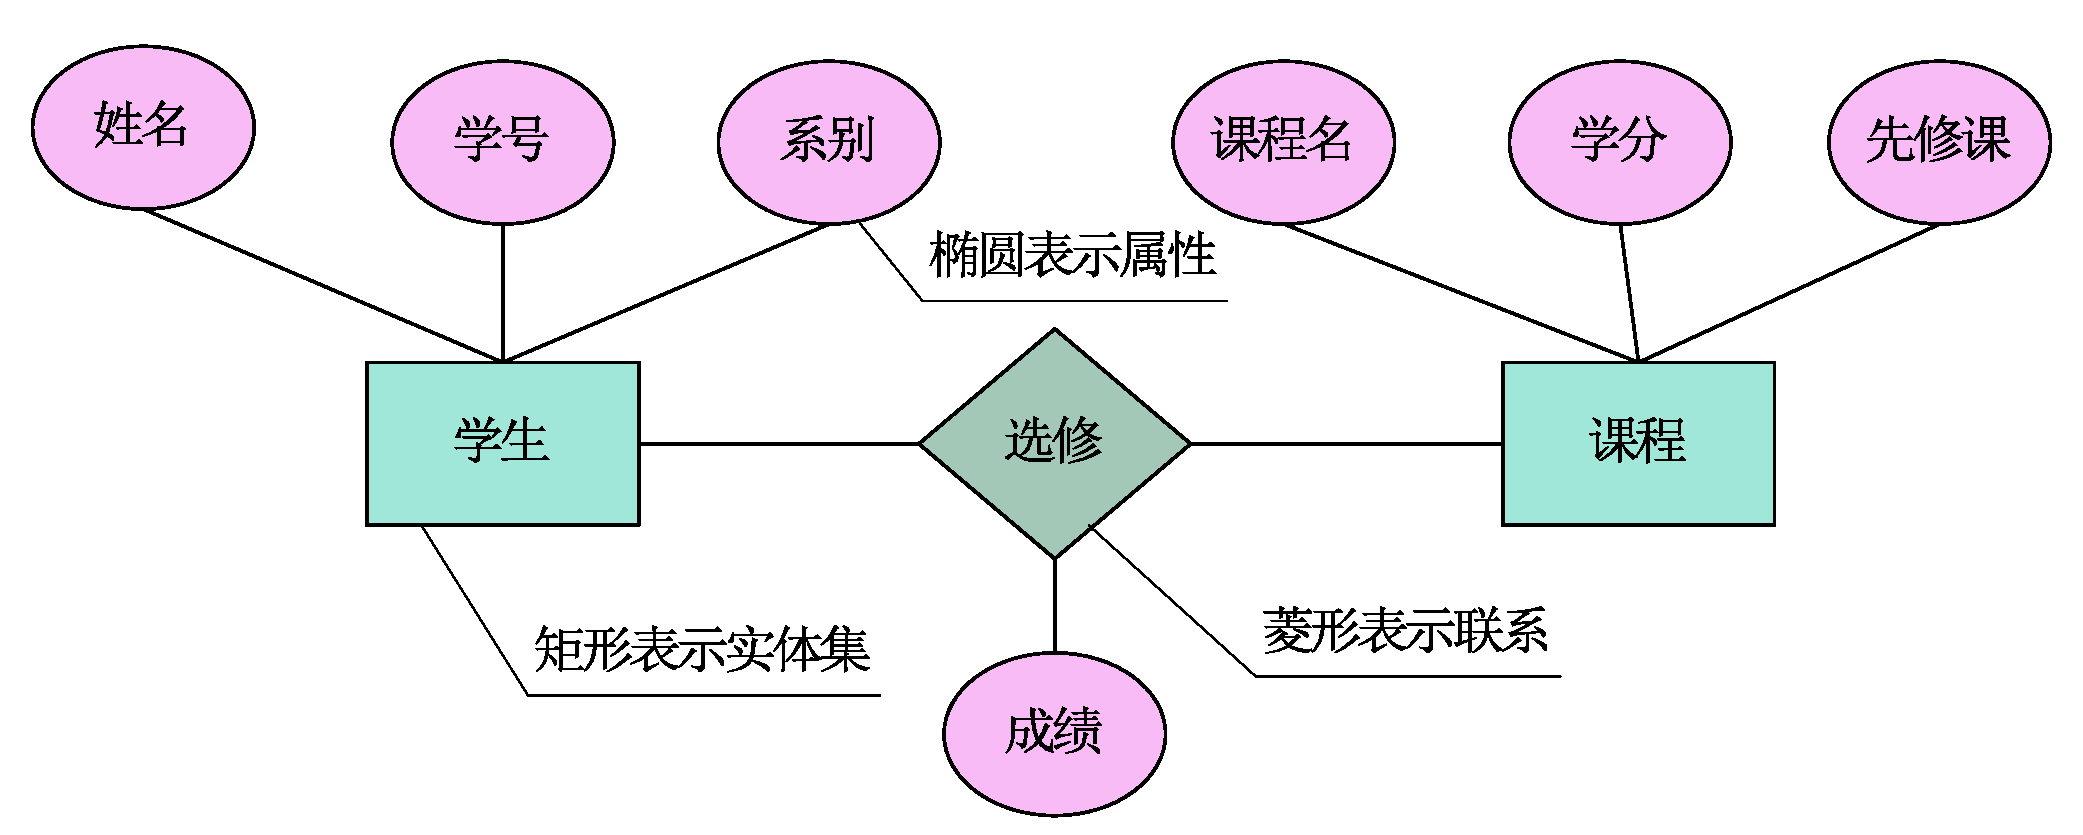
\includegraphics[width=.8\textwidth]{figure/db-8.pdf}
    \caption{E-R图}
\end{figure}

表达一元联系:
\begin{figure}[H]
    \centering
    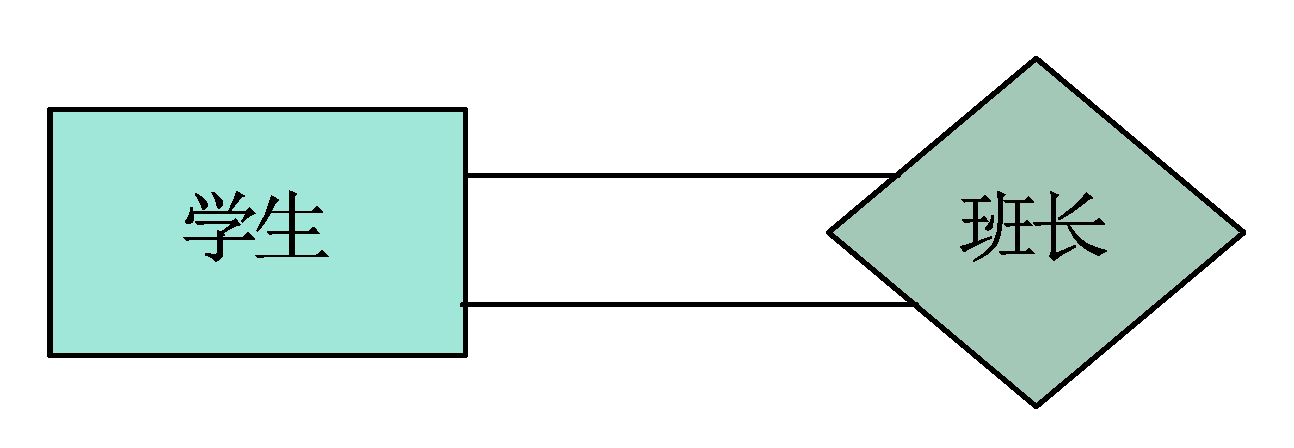
\includegraphics[width=.3\textwidth]{figure/db-9.pdf}
    \caption{一元联系}
\end{figure}

\section{实体的码(Key)}

\begin{definition}[超码(Superkey)]
    能\textcolor{red}{唯一标识实体}的属性或者属性组. 超码的任意超集也是超码.
\end{definition}

\begin{definition}[候选码(candidate key)]
    其任意真子集都不能成为超码的最小超码.
\end{definition}

\begin{definition}[主码(primary key)]
    选定的候选码作为实体的标识码.
\end{definition}

\begin{definition}[替代码]
    除去主码的其他候选码. (可以替代主码的候选码)
\end{definition}

\begin{definition}[代理码]
    人为添加的属性作为主码. e.g. ssn(单纯的随机码)
\end{definition}

\begin{definition}[自然码]
    e.g. 不重名的情况下, 姓名可以作为候选码. “真正的”候选码.
\end{definition}

\begin{definition}[智能码]
    经过编码的标识符. e.g. 学号, 电话号码, 身份证
\end{definition}

\section{属性}

属性包括: 复合、多值、派生、NULL.

\begin{definition}[简单属性]
     不可再分的属性. e.g. 学号, 姓名
\end{definition}

\begin{definition}[复合属性(Composite)]
    可以划分为更小的属性. e.g. 电话号码=区号+号码, 地址=省+市+区+街道+门牌号, 日期=年+月+日.
\end{definition}

\begin{definition}[单值属性]
    每一个特定的实体在该属性上的取值唯一.
\end{definition}

\begin{definition}[多值属性]
    多于一个的取值(取值是一个集合. 必须展开.)
\end{definition}

\begin{definition}[派生属性(Derived)]
    可以从其他属性或者实体派生出来的值. e.g., 绩点可以通过成绩计算出来.
\end{definition}

\begin{definition}[NULL 属性]
    值存在但是目前没有获得其信息. / 当实体在某个属性上没有值时设为 NULL.

    \textcolor{red}{实体完整性: 主码取值不能为 NULL.}
\end{definition}

\begin{figure}[H]
    \centering
    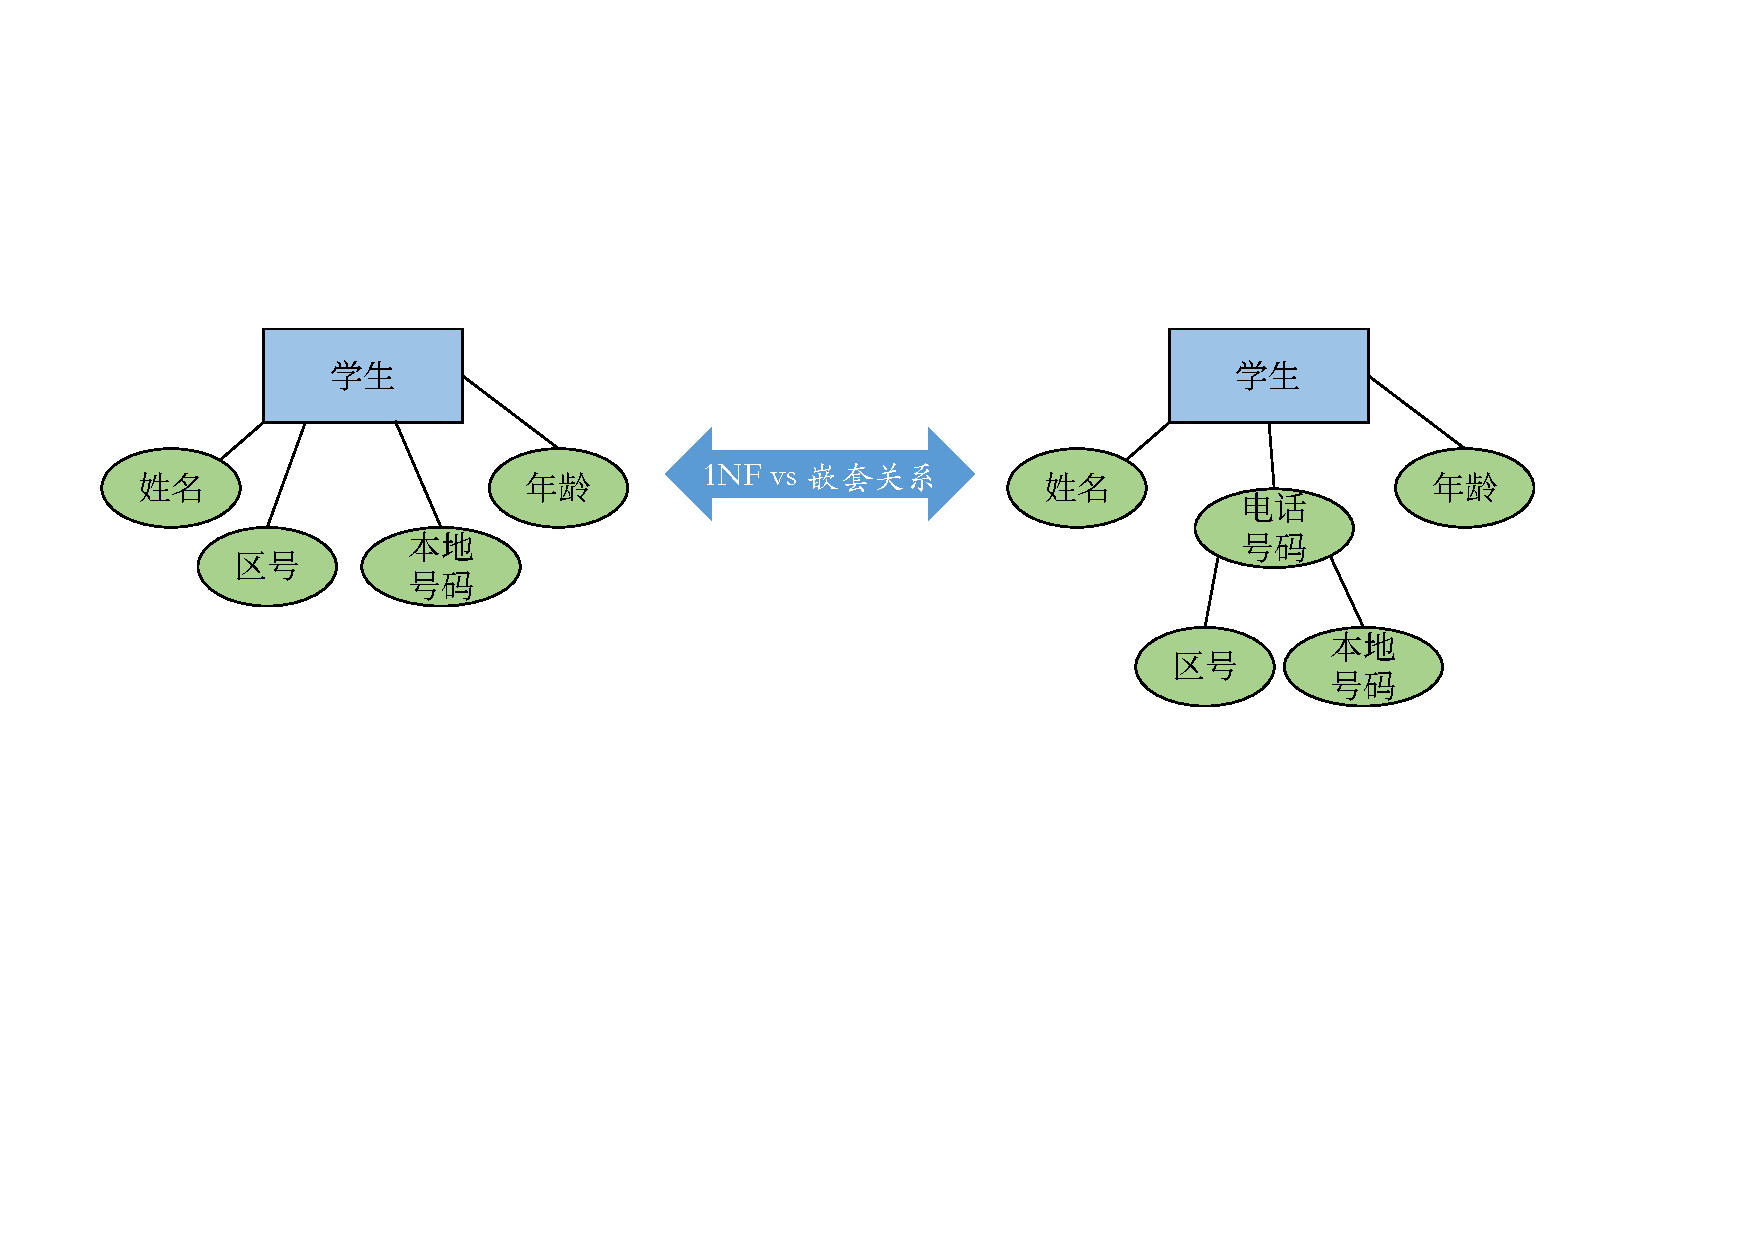
\includegraphics[width=.8\textwidth]{figure/多值.pdf}
    \caption{简单属性 vs 复合属性}
\end{figure}

\begin{figure}[H]
    \centering
    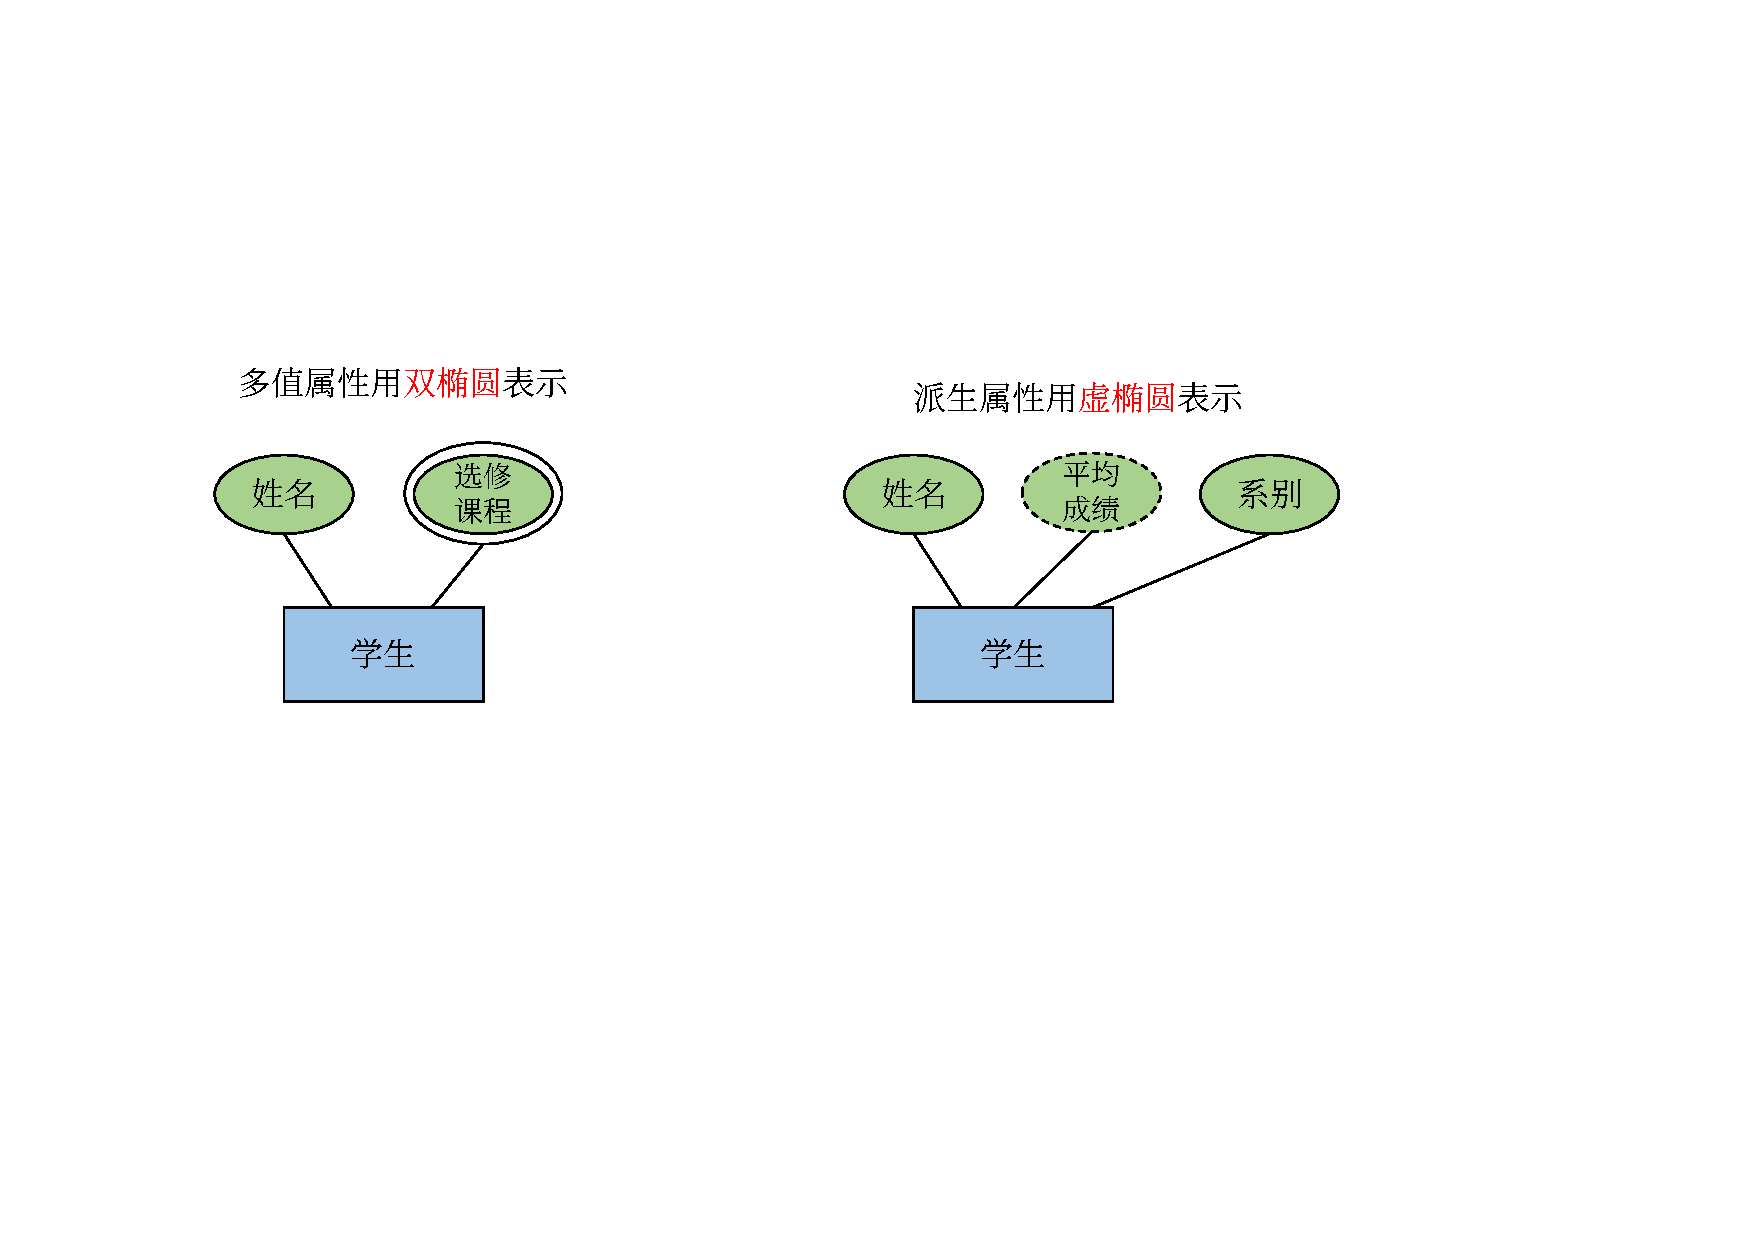
\includegraphics[width=.8\textwidth]{figure/多值属性和派生属性.pdf}
    \caption{多值属性和派生属性的表示}
\end{figure}

\section{联系}

注: 在多方实体和联系之间的线段上标注字母; 在单方实体和联系之间的线段上标注数字1.
\begin{figure}[H]
    \centering
    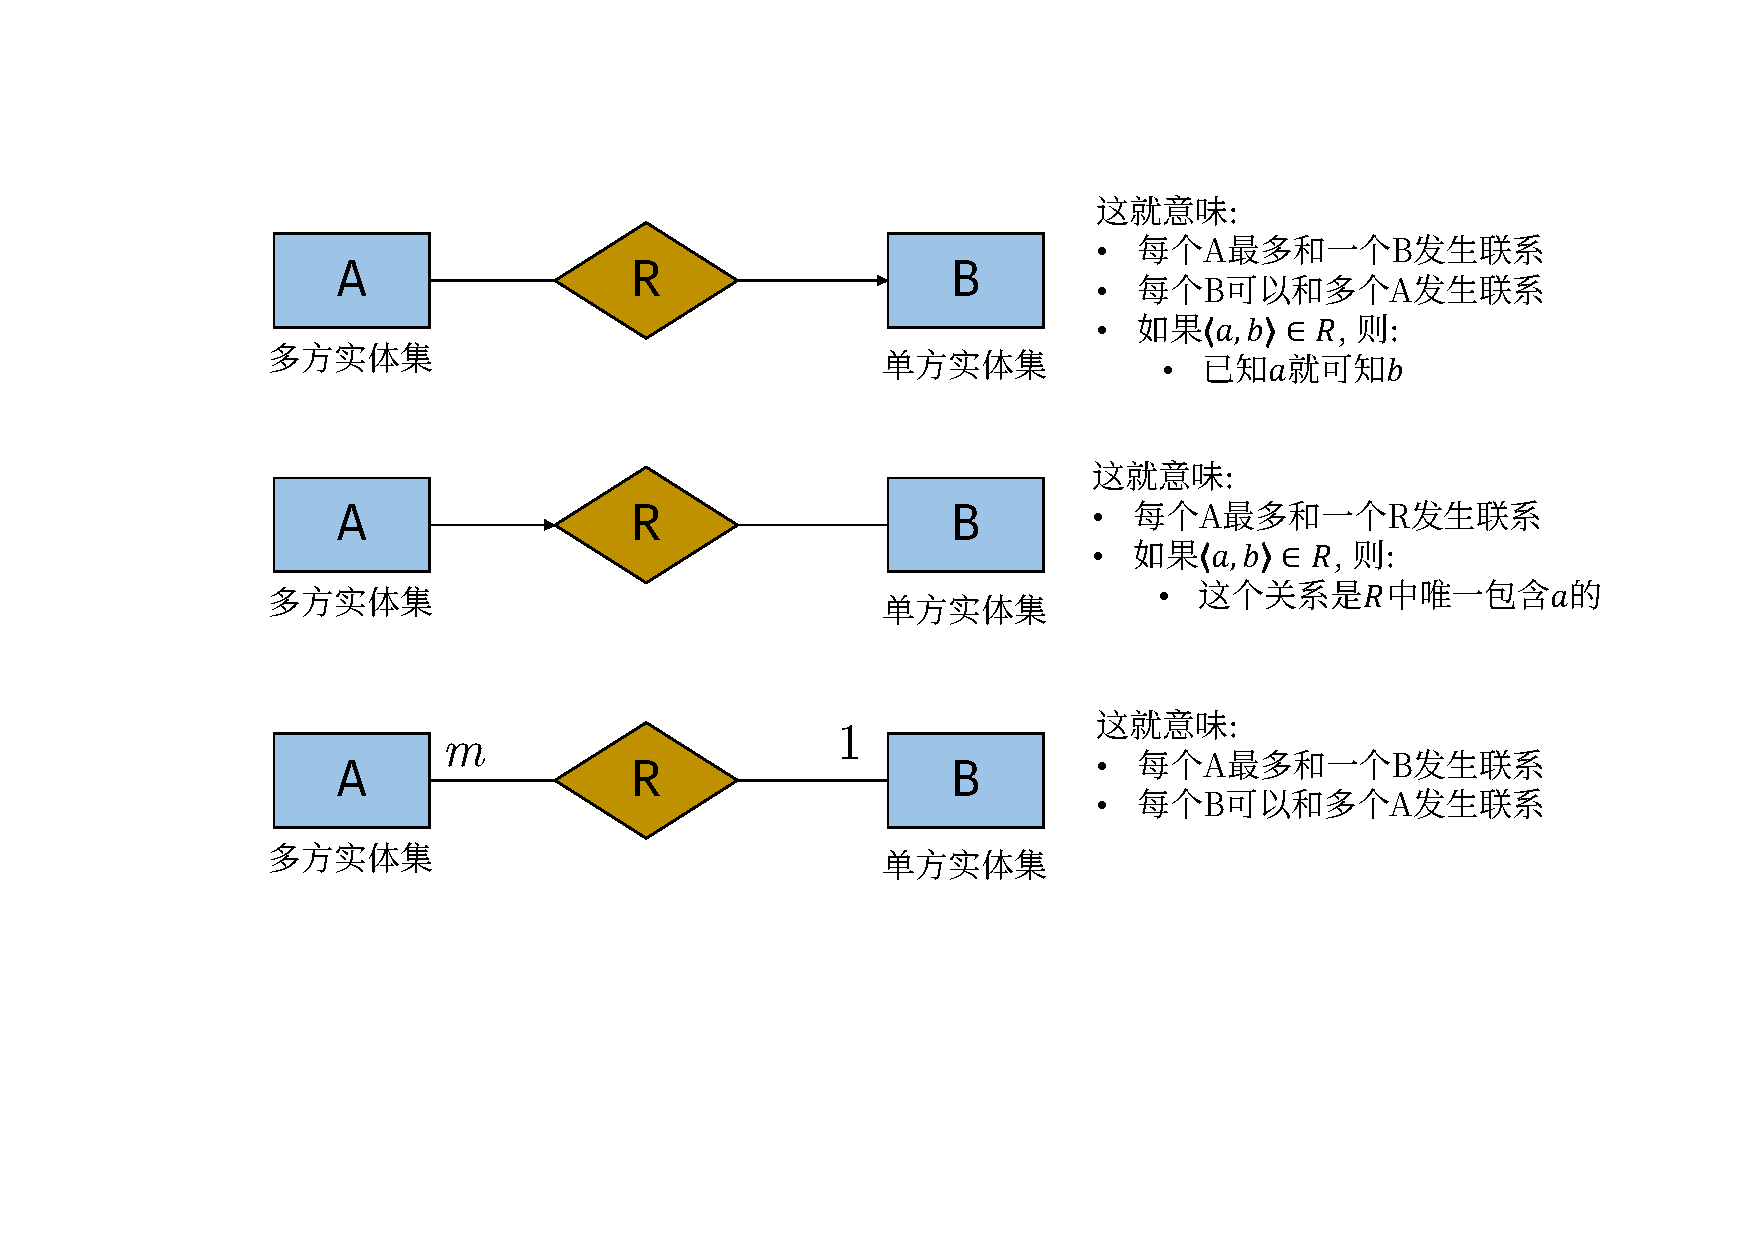
\includegraphics[width=.7\textwidth]{figure/联系.pdf}
    \caption{联系种类在E-R图中的表示}
\end{figure}

\begin{definition}[联系的数量]
    实体之间的\textcolor{red}{联系的数量}, 即一个实体通过一个联系集能与另
    一实体集相关联的实体的数目.
    \begin{itemize}
        \item 一对一的 (1:1)
        \item 一对多的 (1:$m$)
        \item 多对多的 ($m:n$)
    \end{itemize}
\end{definition}

用箭头或线段来表示联系的种类, \textcolor{red}{箭头指向单方实体集}.


二元联系的种类:
\begin{definition}[一对一联系]
    两个实体集$E_1,E_2$之间的一对一联系:
    \begin{itemize}
        \item $E_1$中的一个实体与$E_2$中至多一个实体相联系;
        \item $E_2$中的一个实体与$E_1$中至多一个实体相联系.
    \end{itemize}
    \textcolor{red}{一对一不是一一对应!!!}
\end{definition}

\begin{figure}[H]
    \centering
    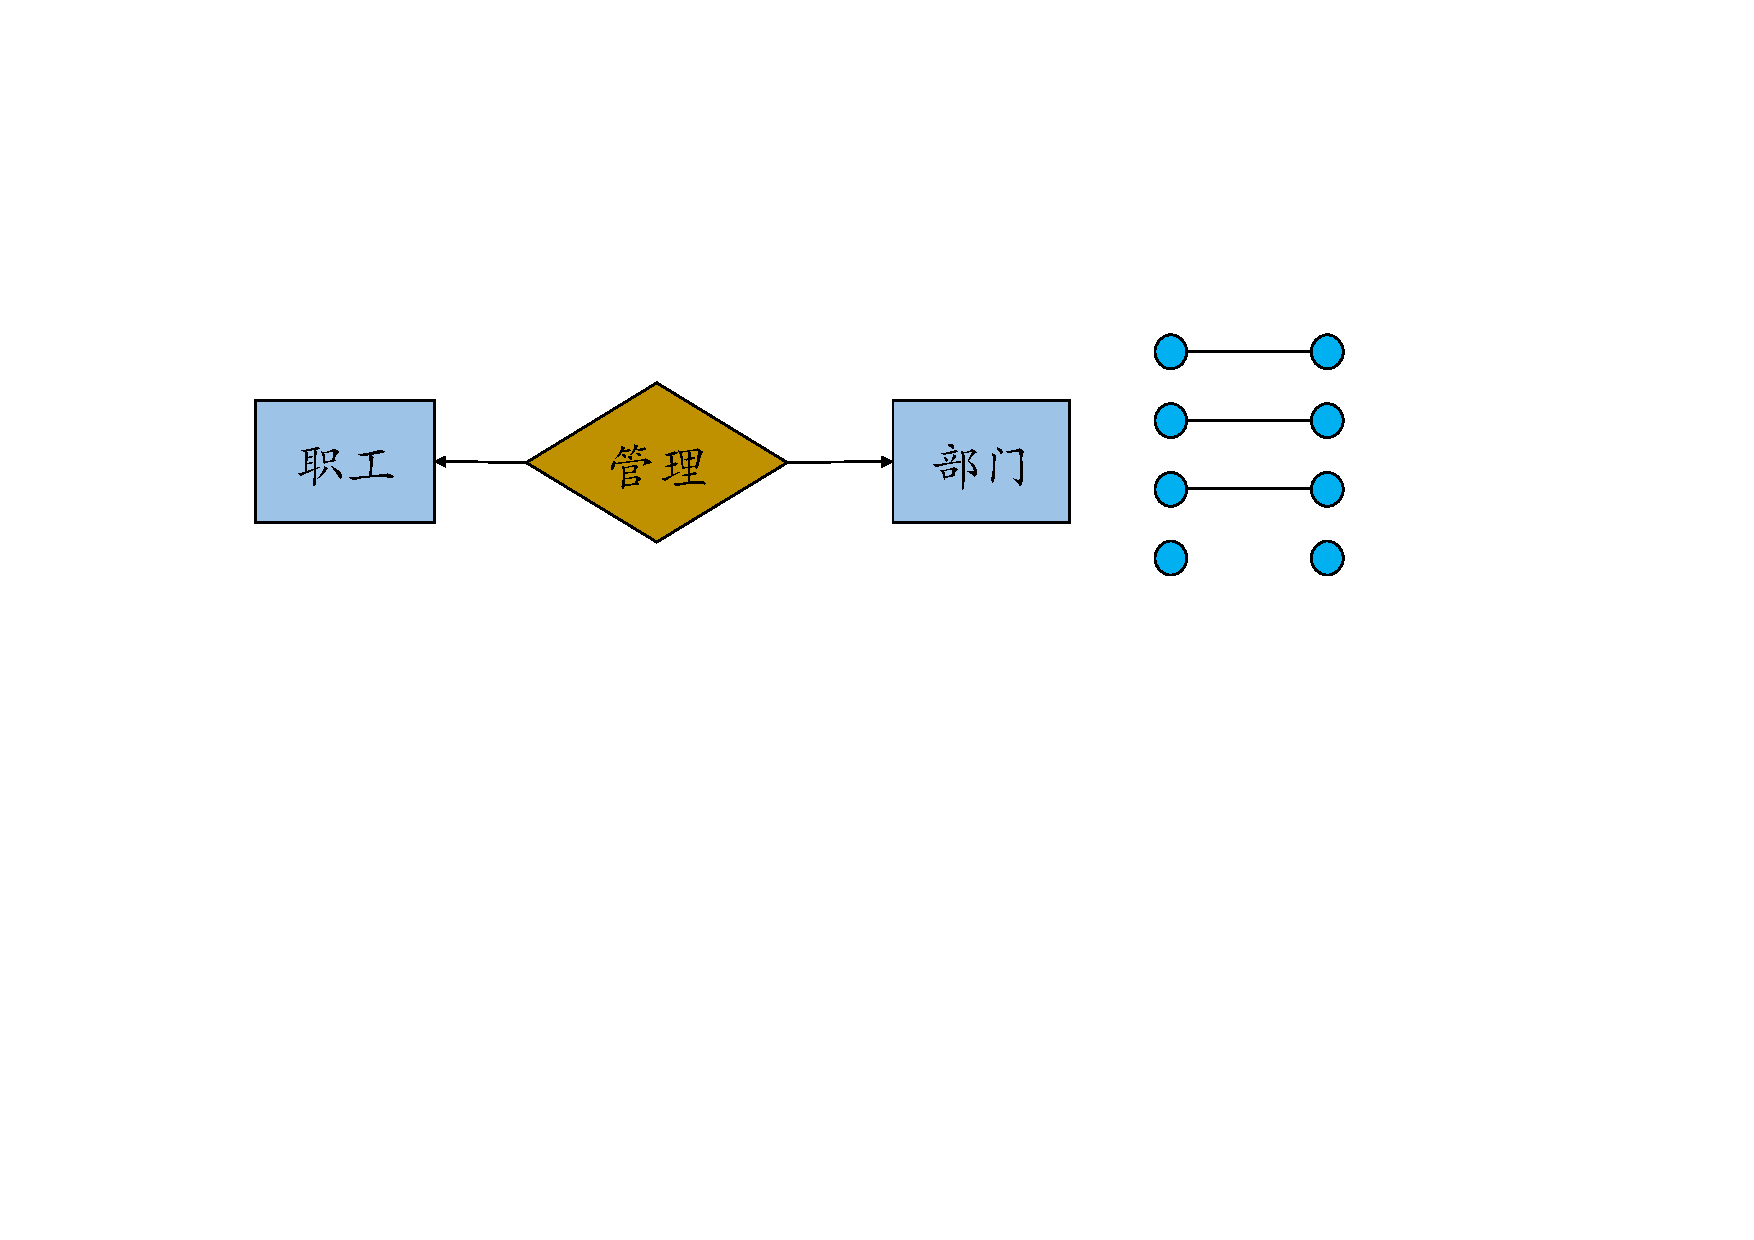
\includegraphics[width=.6\textwidth]{figure/一对一.pdf}
    \caption{一对一联系}
\end{figure}


\begin{definition}[一对多联系]
    两个实体集$E_1,E_2$之间的一对多联系:
    \begin{itemize}
        \item $E_1$中的一个实体与$E_2$中$n(n\geq 0)$个实体相联系;
        \item $E_2$中的一个实体与$E_1$中至多一个实体相联系.
    \end{itemize}
\end{definition}

\begin{figure}[H]
    \centering
    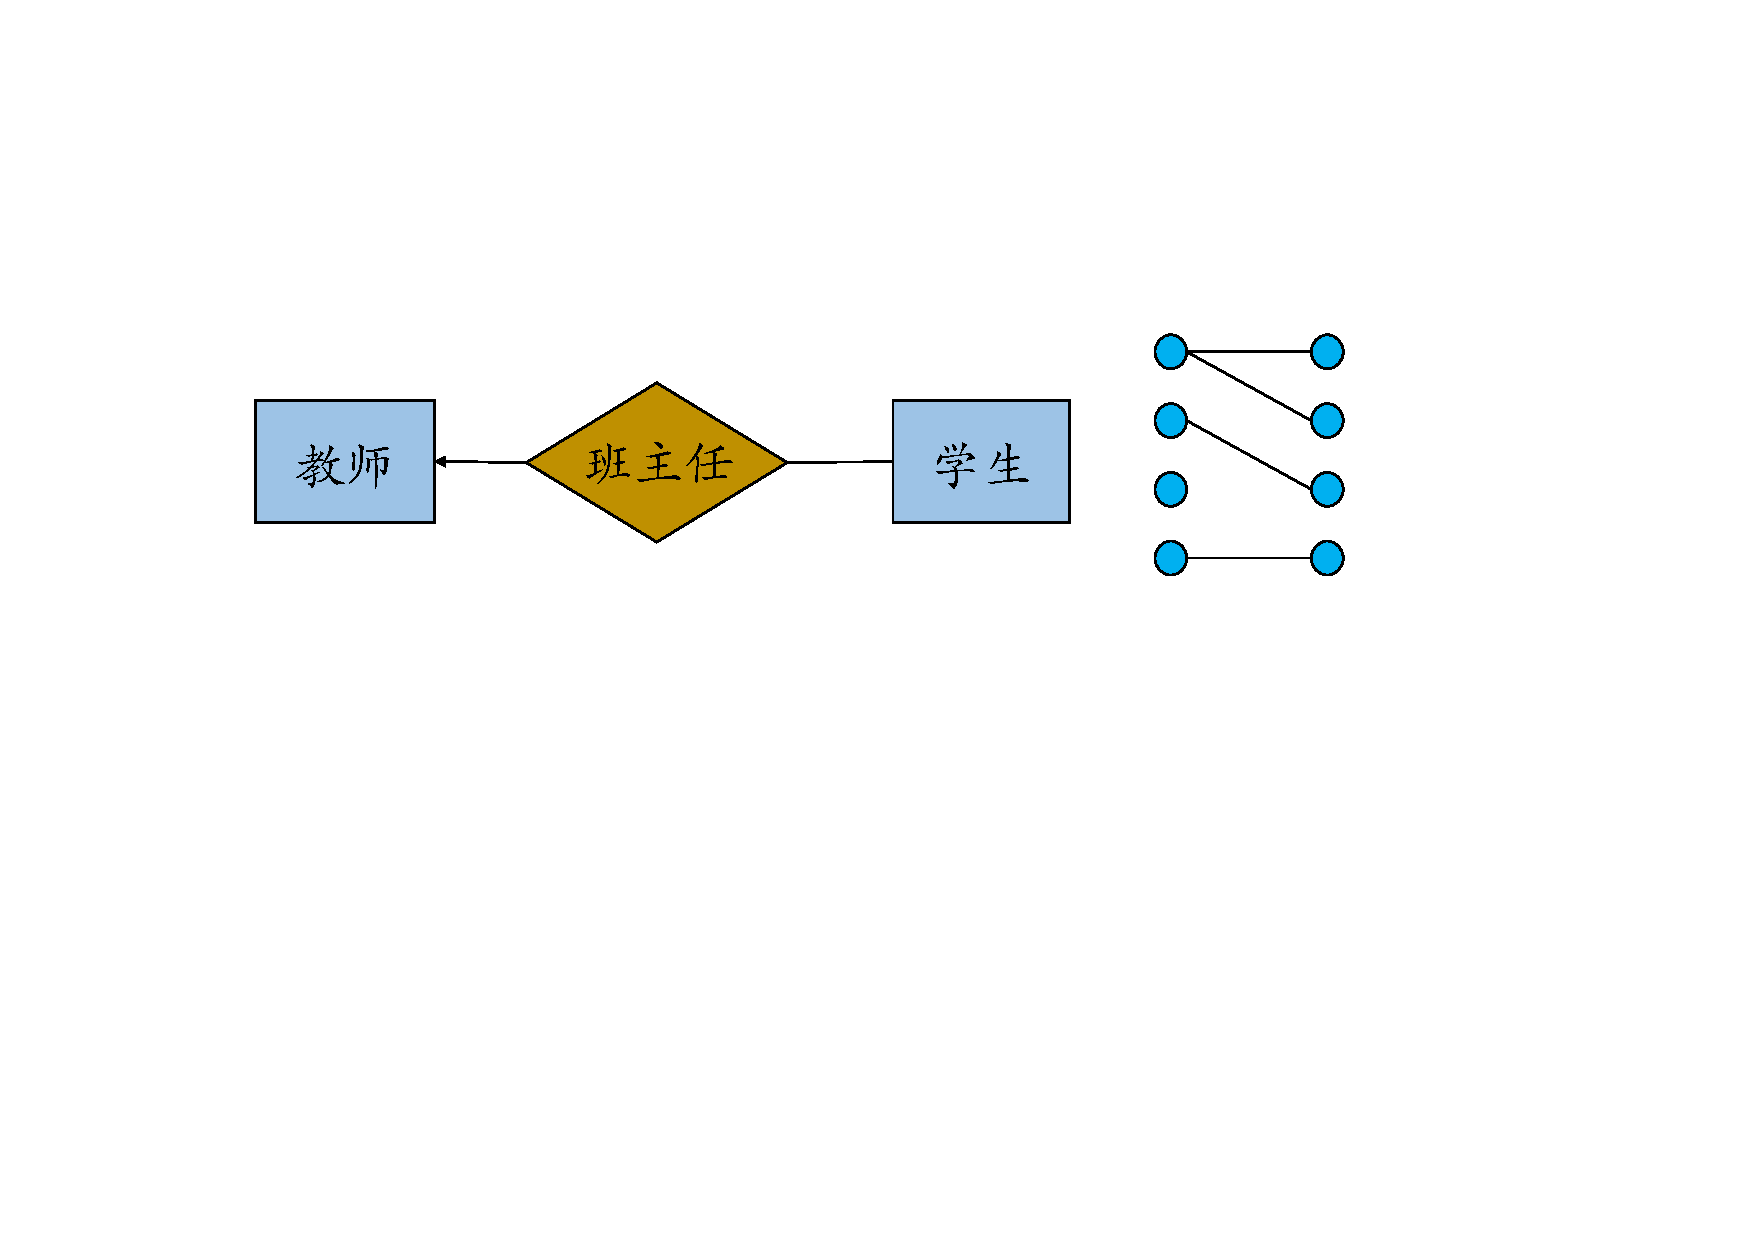
\includegraphics[width=.6\textwidth]{figure/一对多.pdf}
    \caption{一对多联系}
\end{figure}

\begin{definition}[多对多联系]
    两个实体集$E_1,E_2$之间的多对多联系:
    \begin{itemize}
        \item $E_1$中的一个实体与$E_2$中$n(n\geq 0)$个实体相联系;
        \item $E_2$中的一个实体与$E_1$中$m(m\geq 0)$个实体相联系.
    \end{itemize}
\end{definition}

\begin{figure}[H]
    \centering
    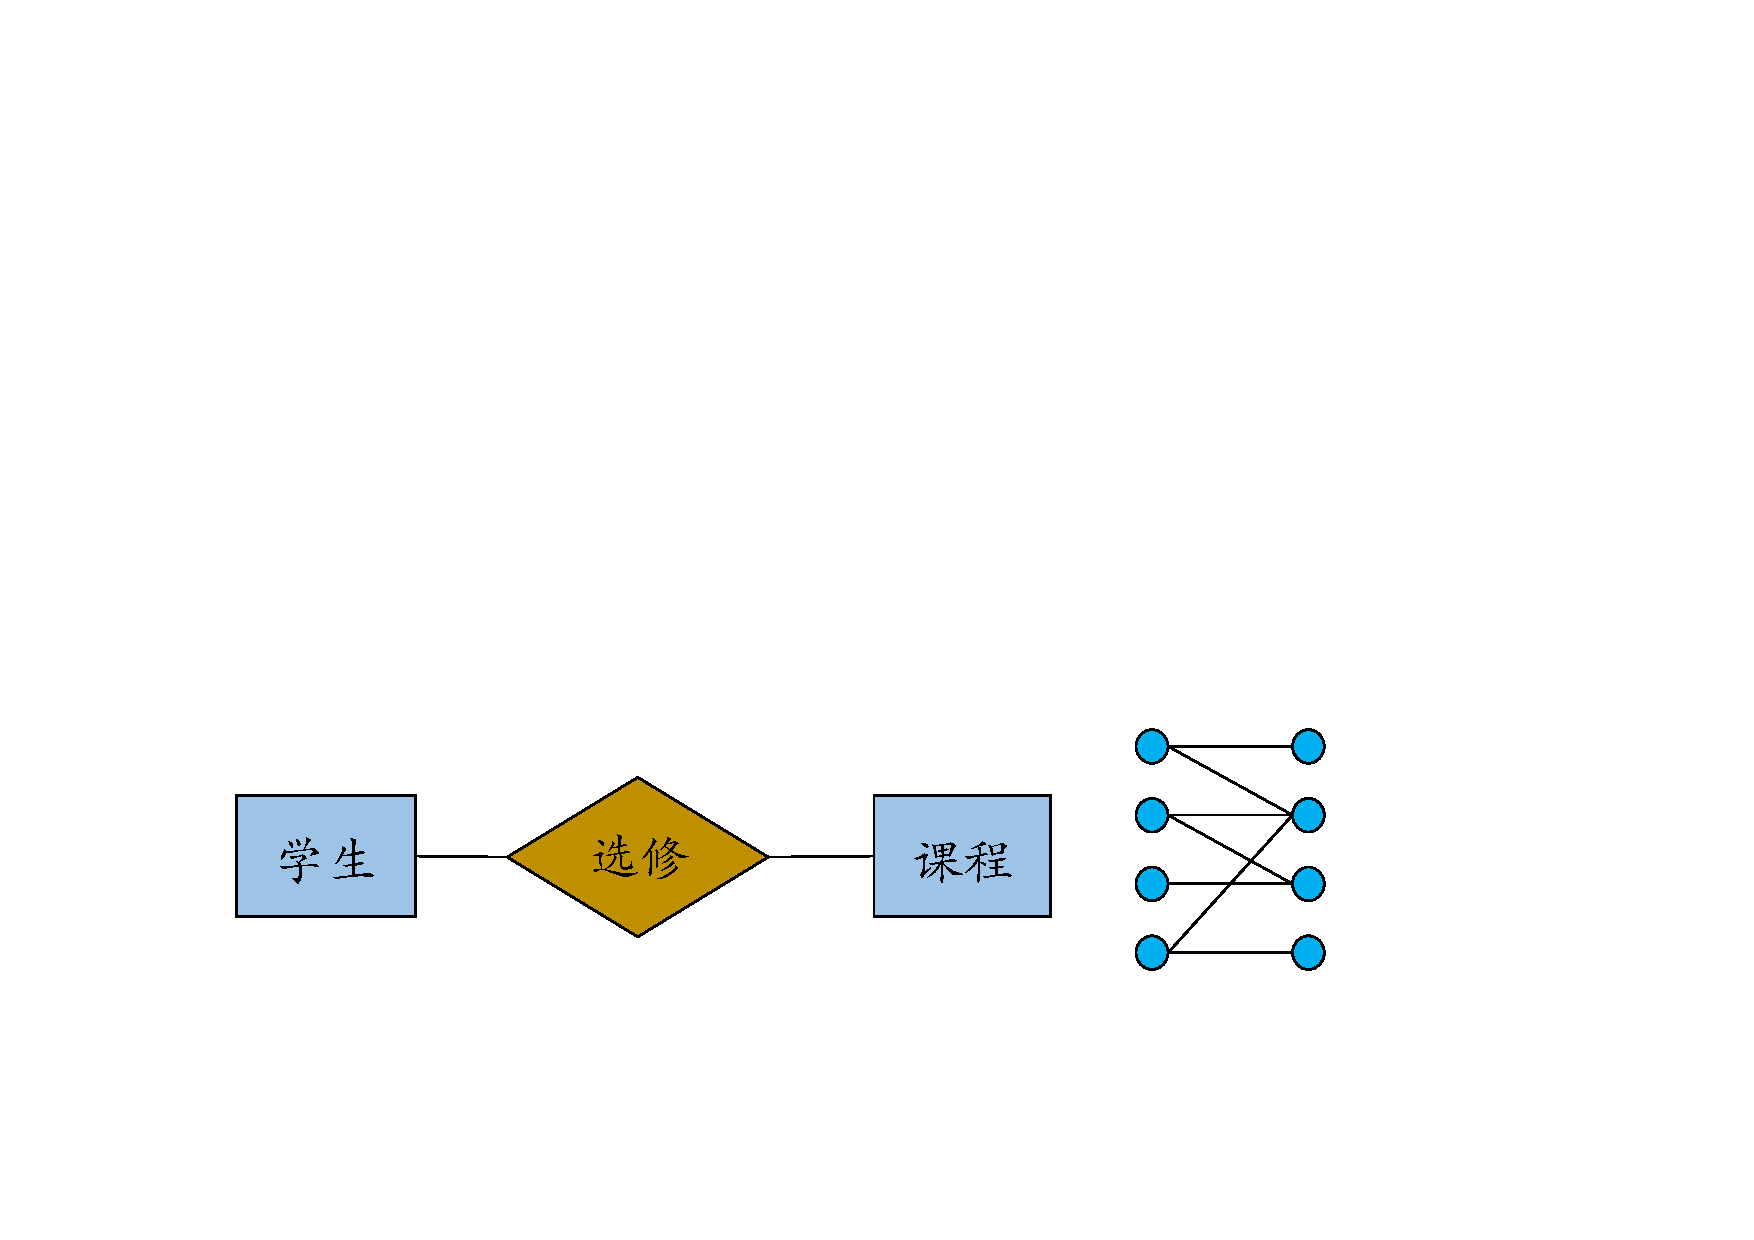
\includegraphics[width=.6\textwidth]{figure/多对多.pdf}
    \caption{多对多联系}
\end{figure}

\textbf{一个实体集内的递归联系:}

\begin{figure}[H]
    \centering
    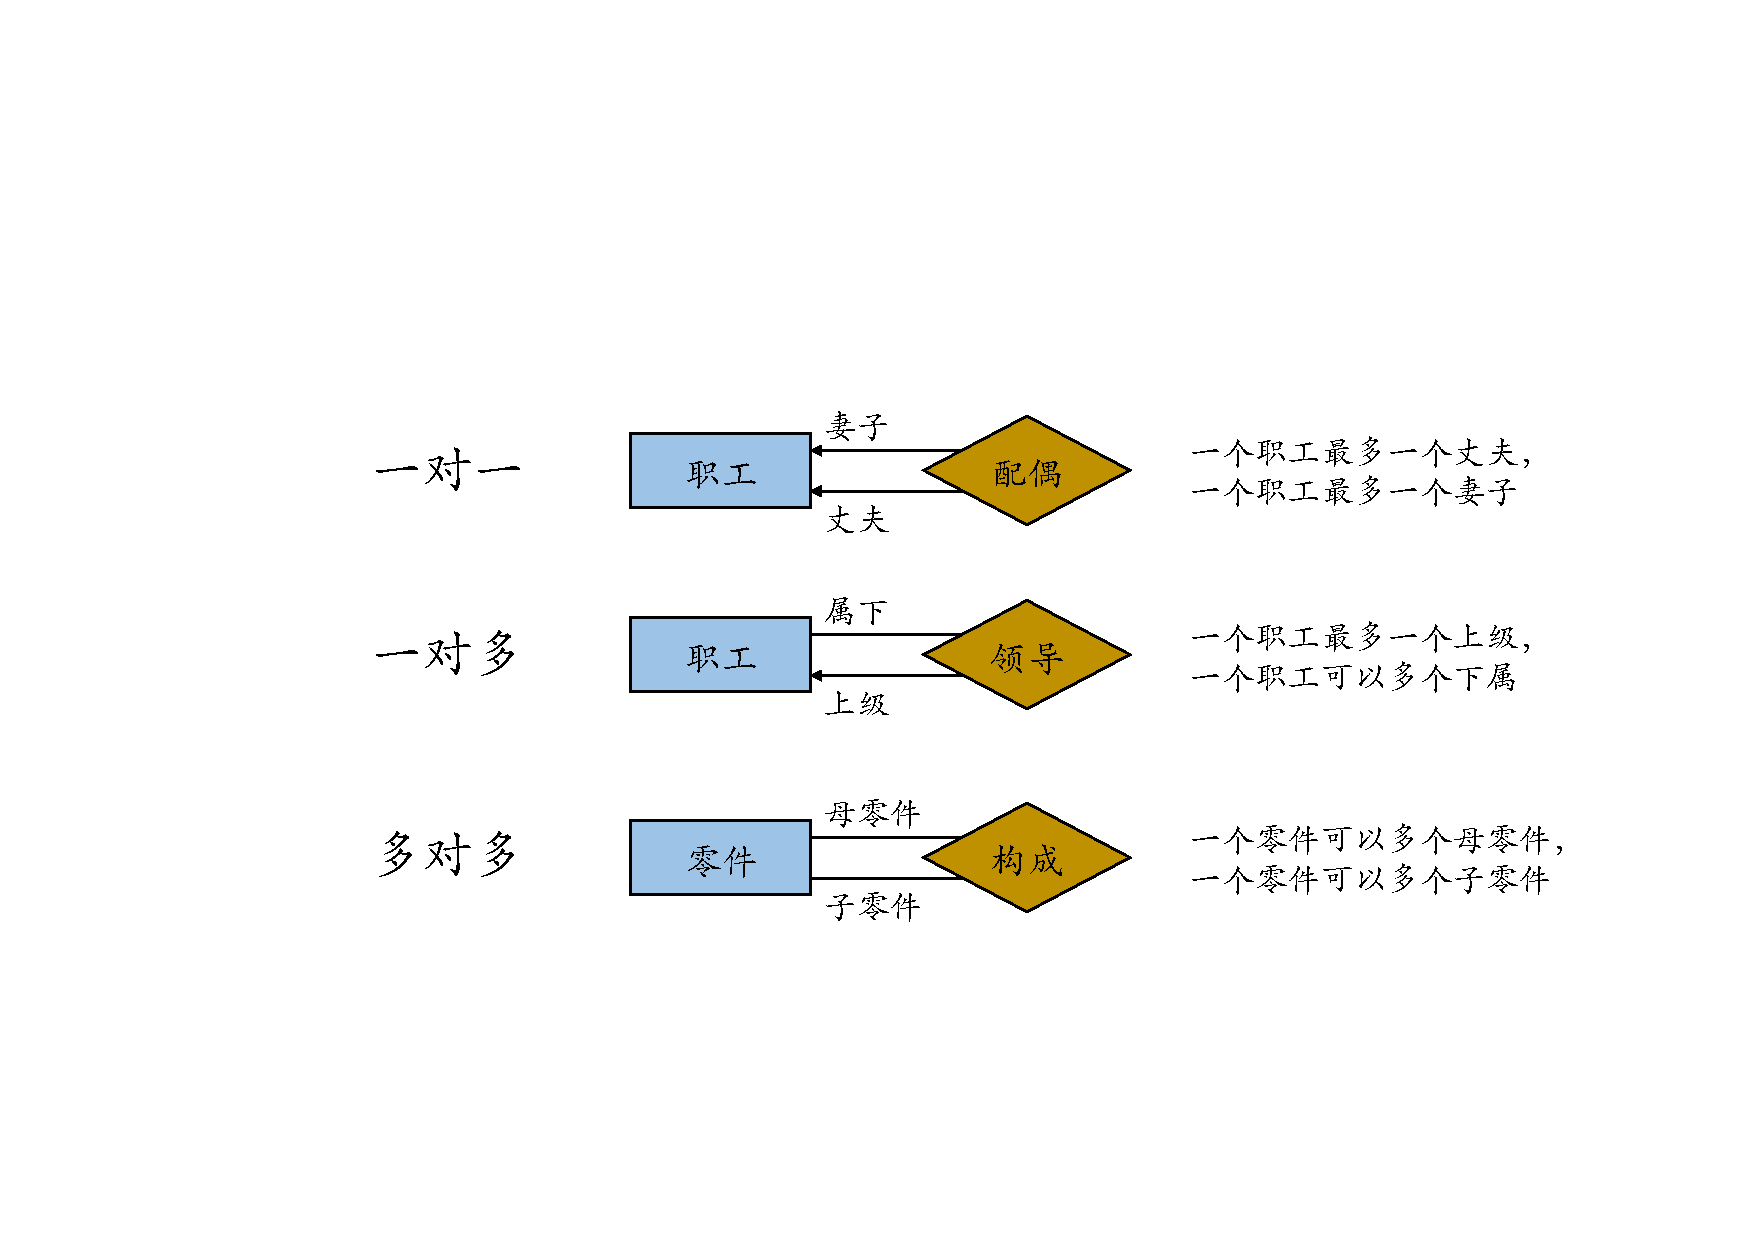
\includegraphics[width=.7\textwidth]{figure/递归联系.pdf}
    \caption{一个实体集内的递归联系}
    \label{n-ary-link}
\end{figure}

\begin{definition}[多元联系]
    当一个联系涉及三个或更多实体集时, 我们称之为多元联系.
\end{definition}

\begin{figure}[H]
    \centering
    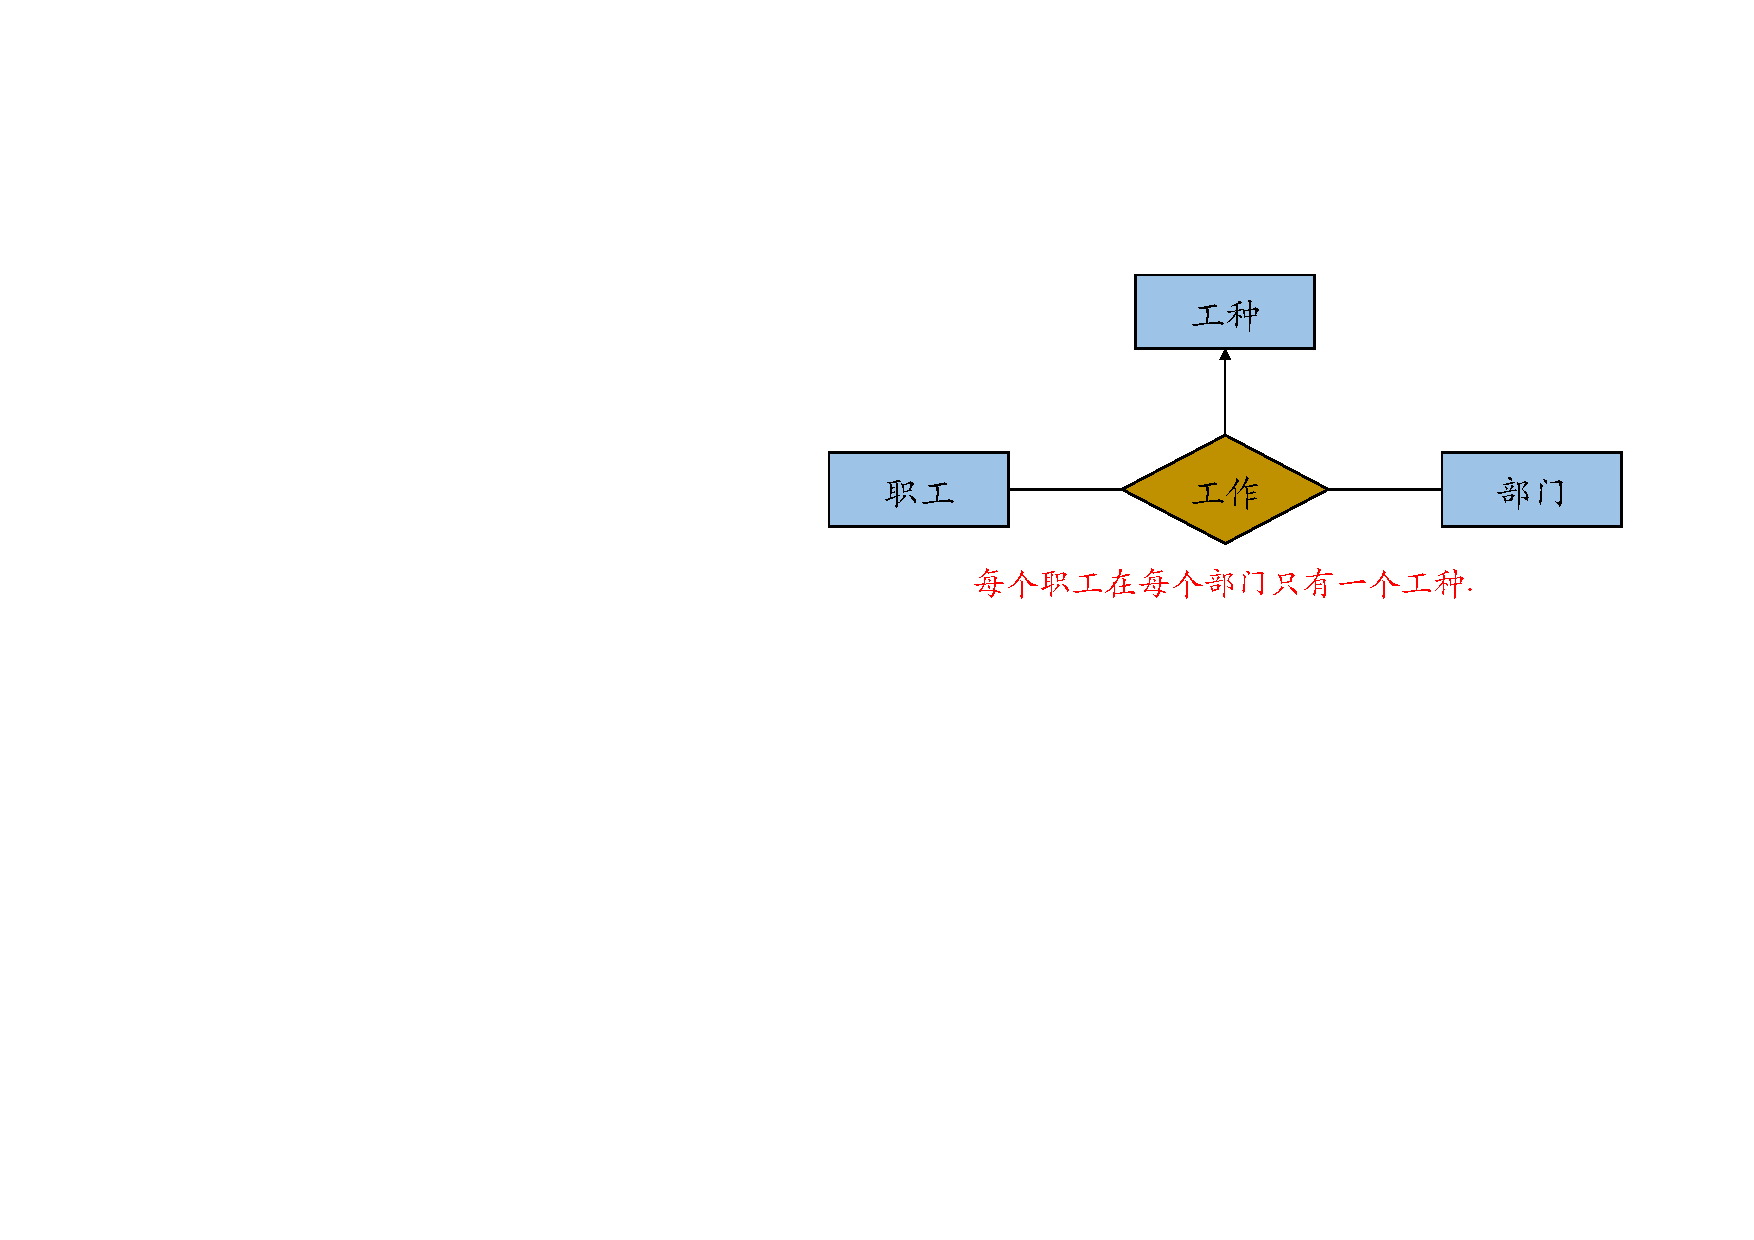
\includegraphics[width=.5\textwidth]{figure/多元联系.pdf}
    \caption{多元联系}
\end{figure}

\begin{definition}[联系的势]
    势表达了一个实体出现在联系中的次数.
\end{definition}

\begin{figure}[H]
    \centering
    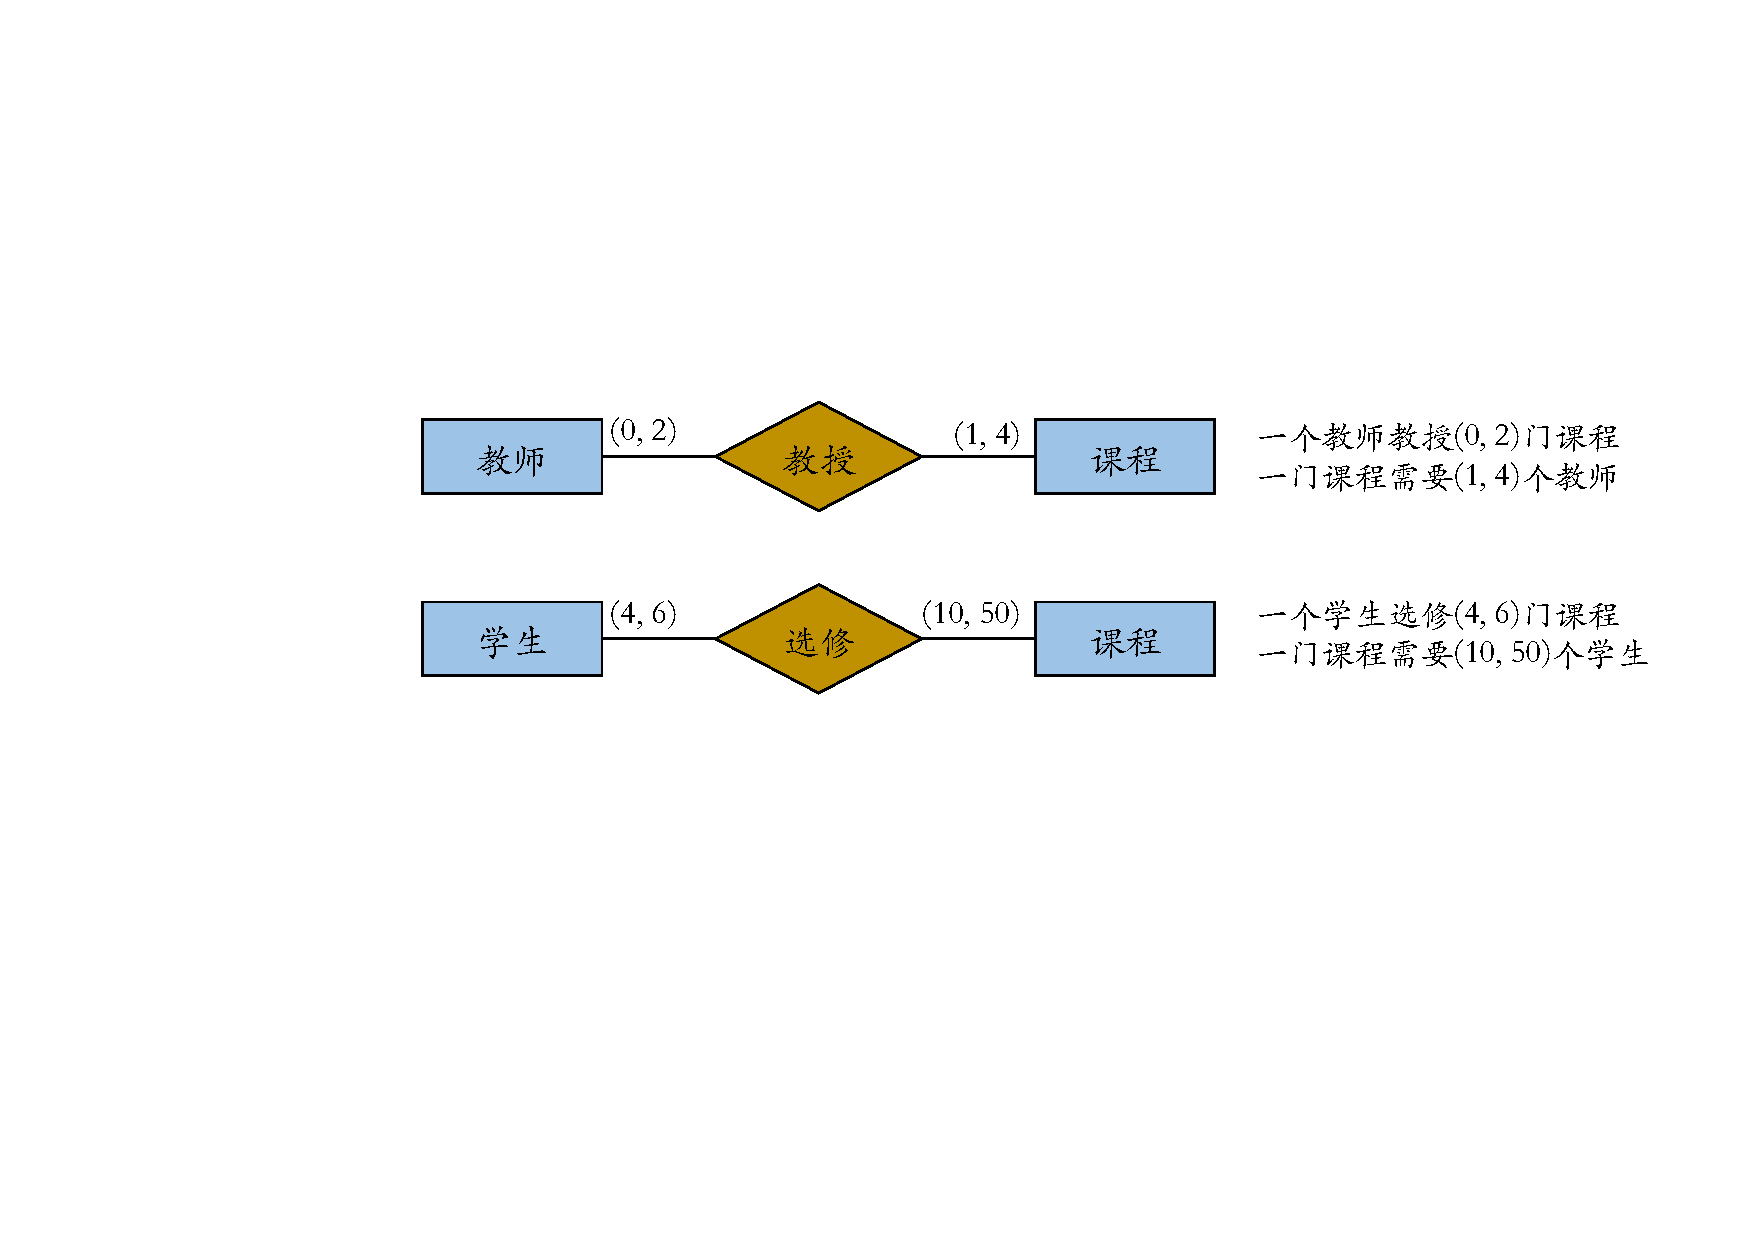
\includegraphics[width=.8\textwidth]{figure/联系的势.pdf}
    \caption{联系的势}
\end{figure}

\section{ER设计实例}

\subsection{基于业务描述的ER设计实例}

\begin{example}
    考虑一个学校数据库, 它要存储以下信息:
    \begin{itemize}
        \item 教师: \underline{教工号}、教工名、职称;
        \item 项目: \underline{项目号}、项目名称、起始年份、资助额;
        \item 学生: \underline{学号}、学生名、年龄、学位;
        \item 一个教工可以负责多个项目;
        \item 每个项目只能有一个负责人;
        \item 一个老师可以参与多个项目;
        \item 一个学生只能参与一个项目;
        \item 一个项目可以有多个学生和老师参与.
    \end{itemize}
\end{example}

\begin{figure}[H]
    \centering
    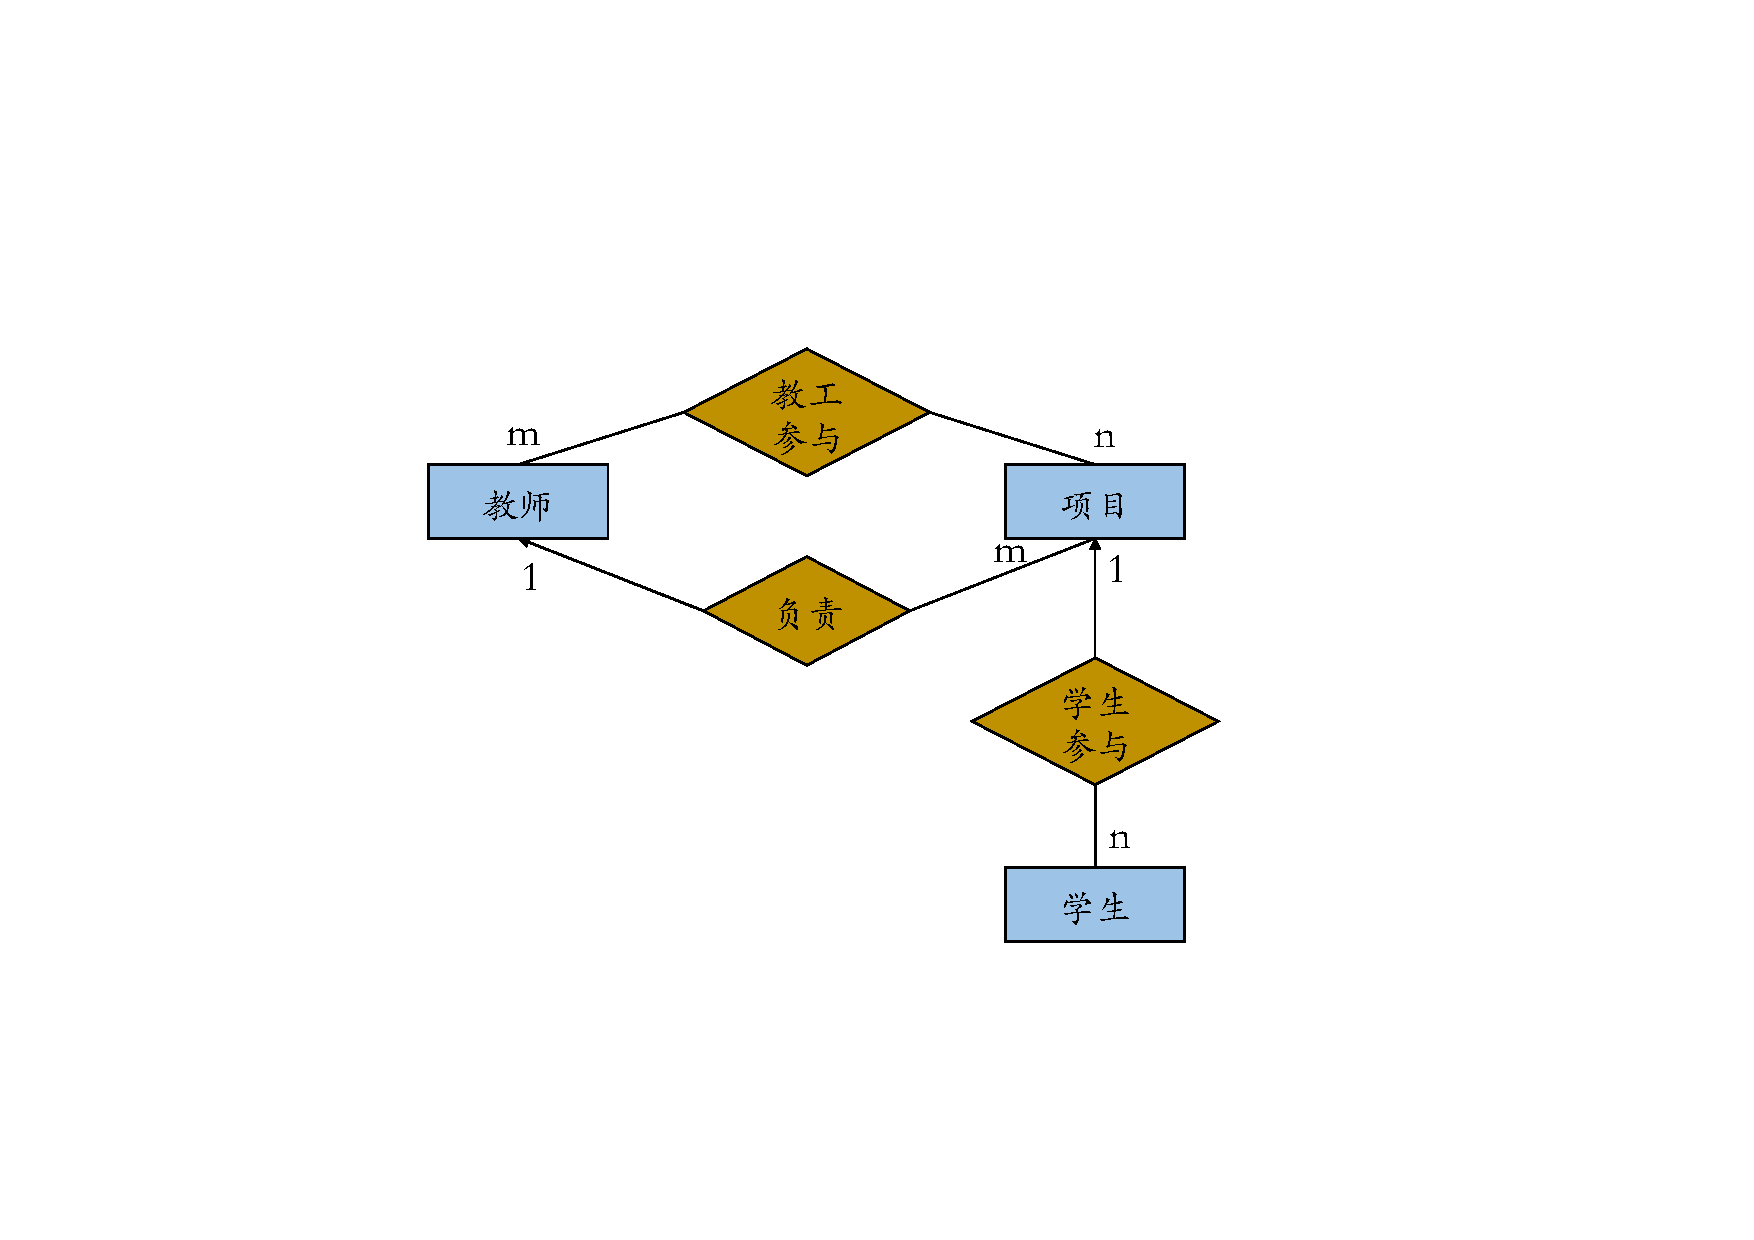
\includegraphics[width=.5\textwidth]{figure/ER实例1.pdf}
    \caption{基于业务描述的ER设计实例}
\end{figure}

\subsection{由业务单据生成ER模型}

\begin{figure}[H]
    \centering
    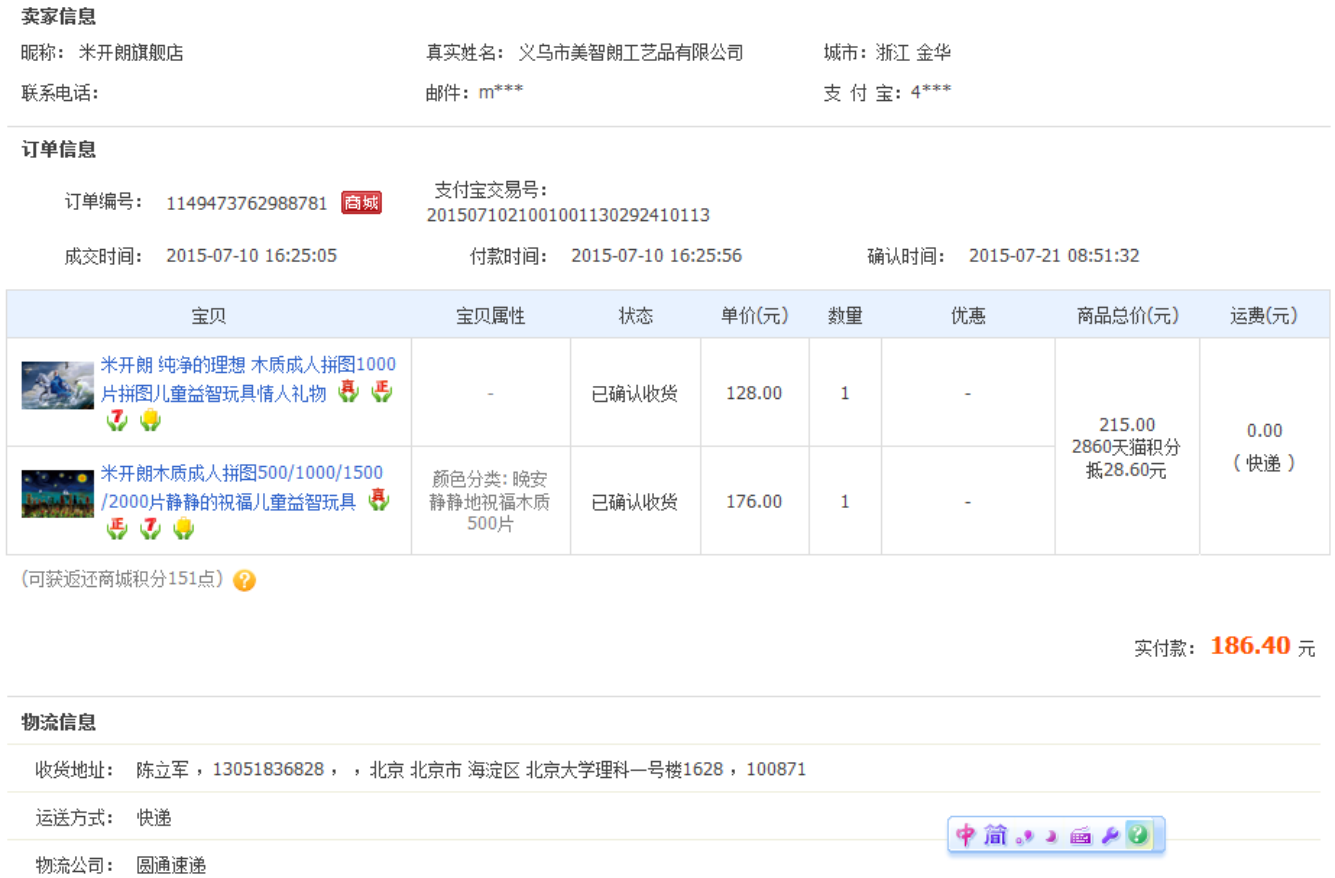
\includegraphics[width=.7\textwidth]{figure/ER实例2.png}
    \caption{订单}
\end{figure}

\begin{figure}[H]
    \centering
    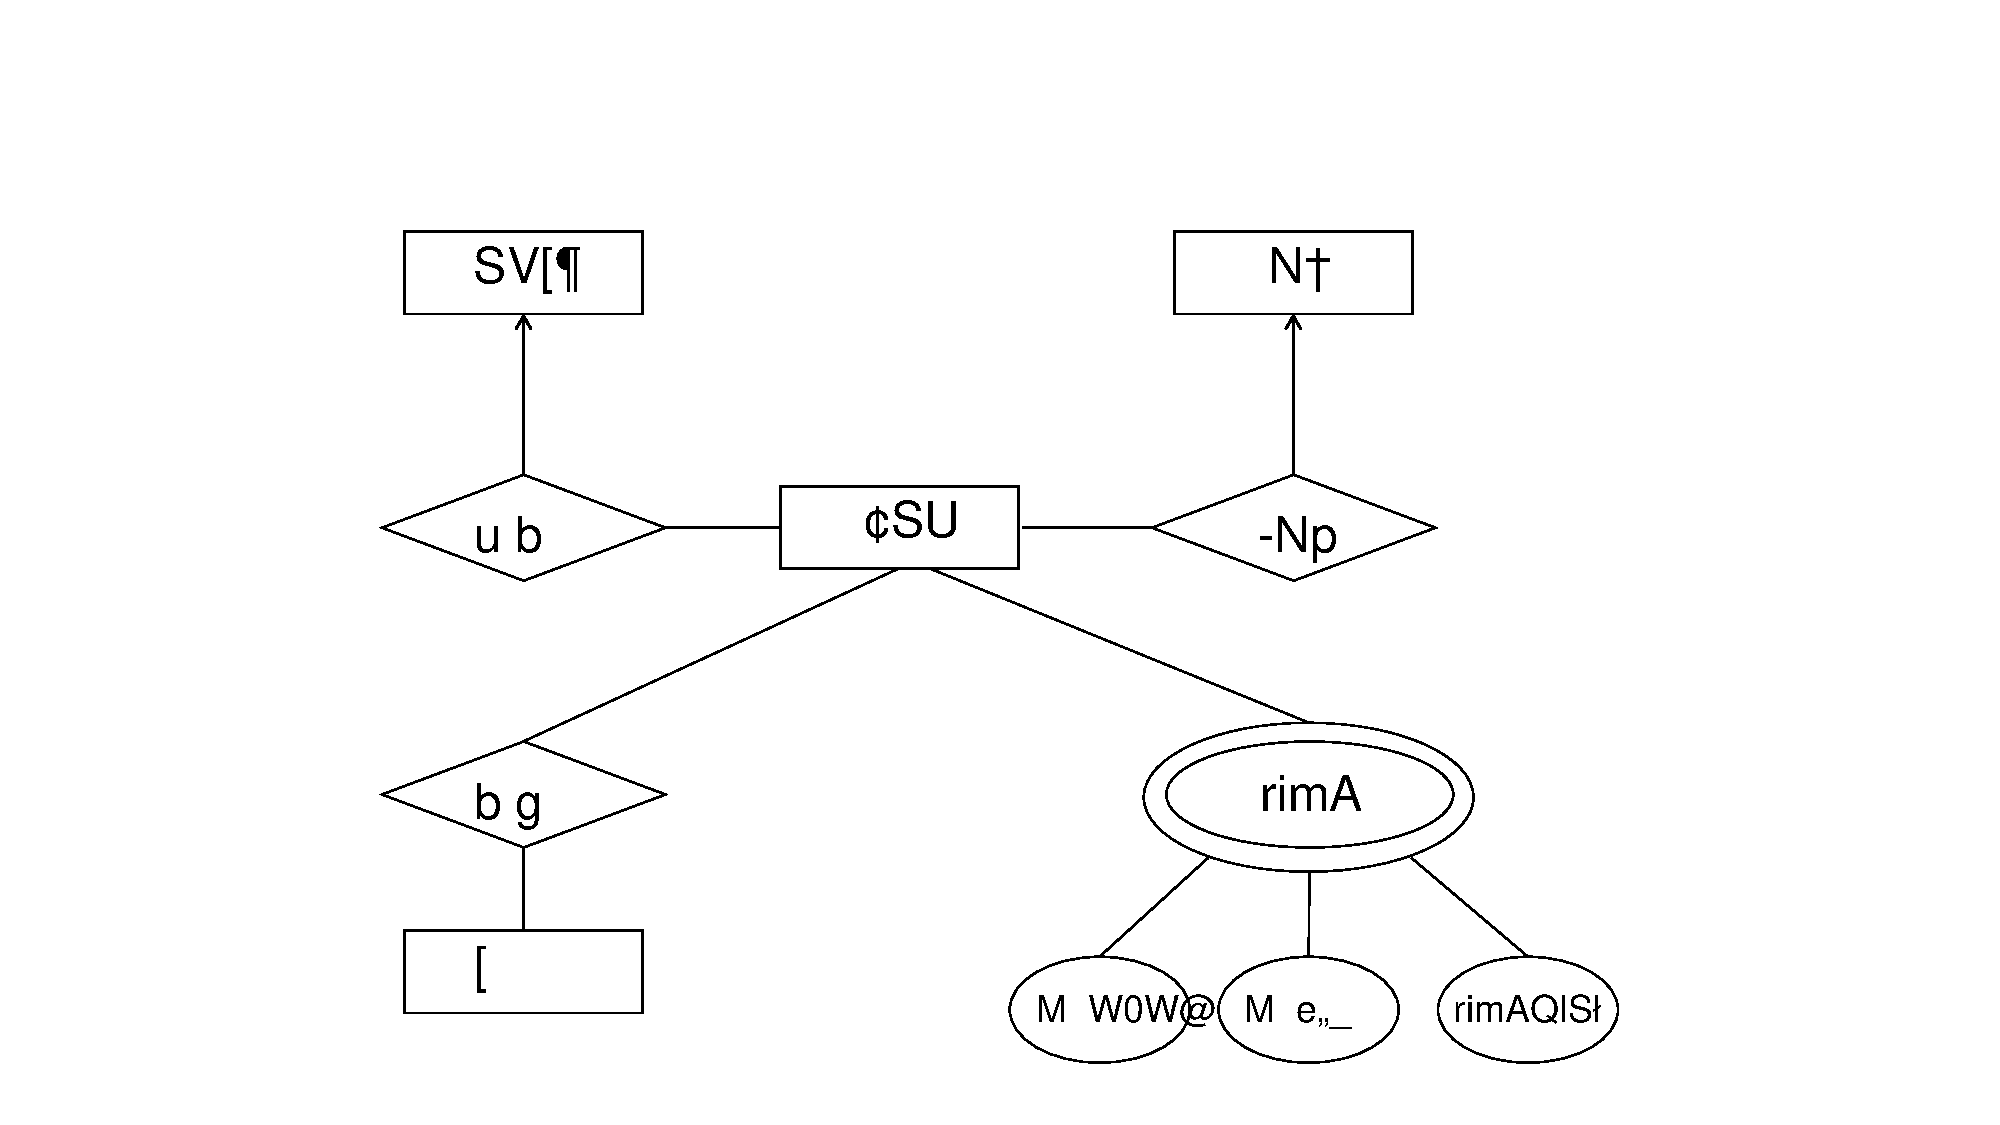
\includegraphics[width=.6\textwidth]{figure/ER实例3.pdf}
    \caption{由业务单据生成ER模型}
\end{figure}

\section{其他概念术语}

\begin{definition}[参与 (Participation)]
    实体集之间的关联称为参与, 即实体参与联系.
    \begin{itemize}
        \item $E$全部参与$R$: 实体集$E$中的每个实体都参与到联系集$R$中的至少一个联系.
        \item $E$部分参与$R$: 实体集$E$中只有部分实体参与到联系集$R$中的联系.
    \end{itemize}
\end{definition}

\begin{figure}[H]
    \centering
    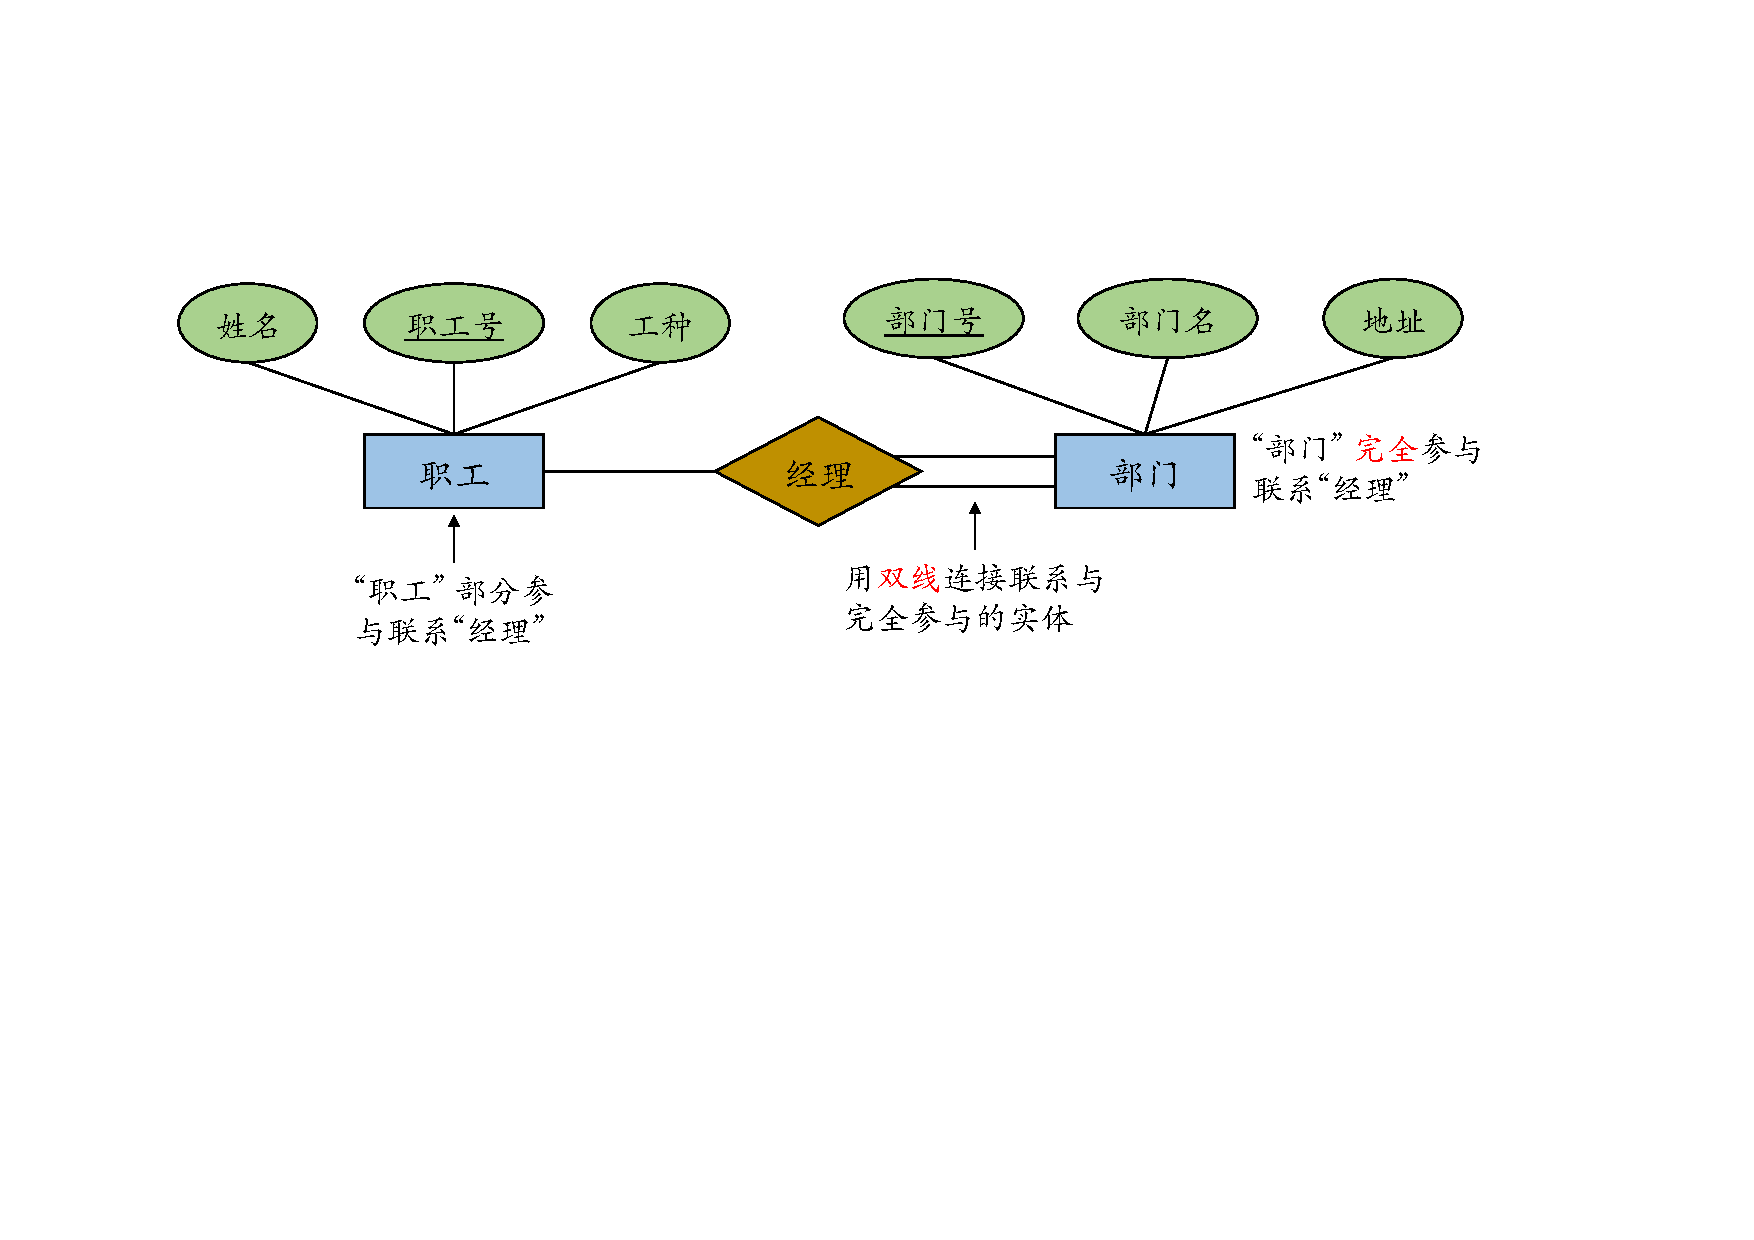
\includegraphics[width=.8\textwidth]{figure/参与.pdf}
    \caption{参与的ER图表示}
\end{figure}

\begin{definition}[角色 (Role)]
    实体在联系中的作用称为实体的角色. 对于一元联系, 为区别各实体参与联系的方式, 需要显式指明其角色. 如图\ref{n-ary-link}.
\end{definition}

\begin{definition}[存在依赖 (Exisitence Dependency)]
    $x$存在依赖于$y$意味着实体$x$的存在依赖于$y$, $y$称为支配实体, $x$称为从属实体.
\end{definition}

\begin{figure}[H]
    \centering
    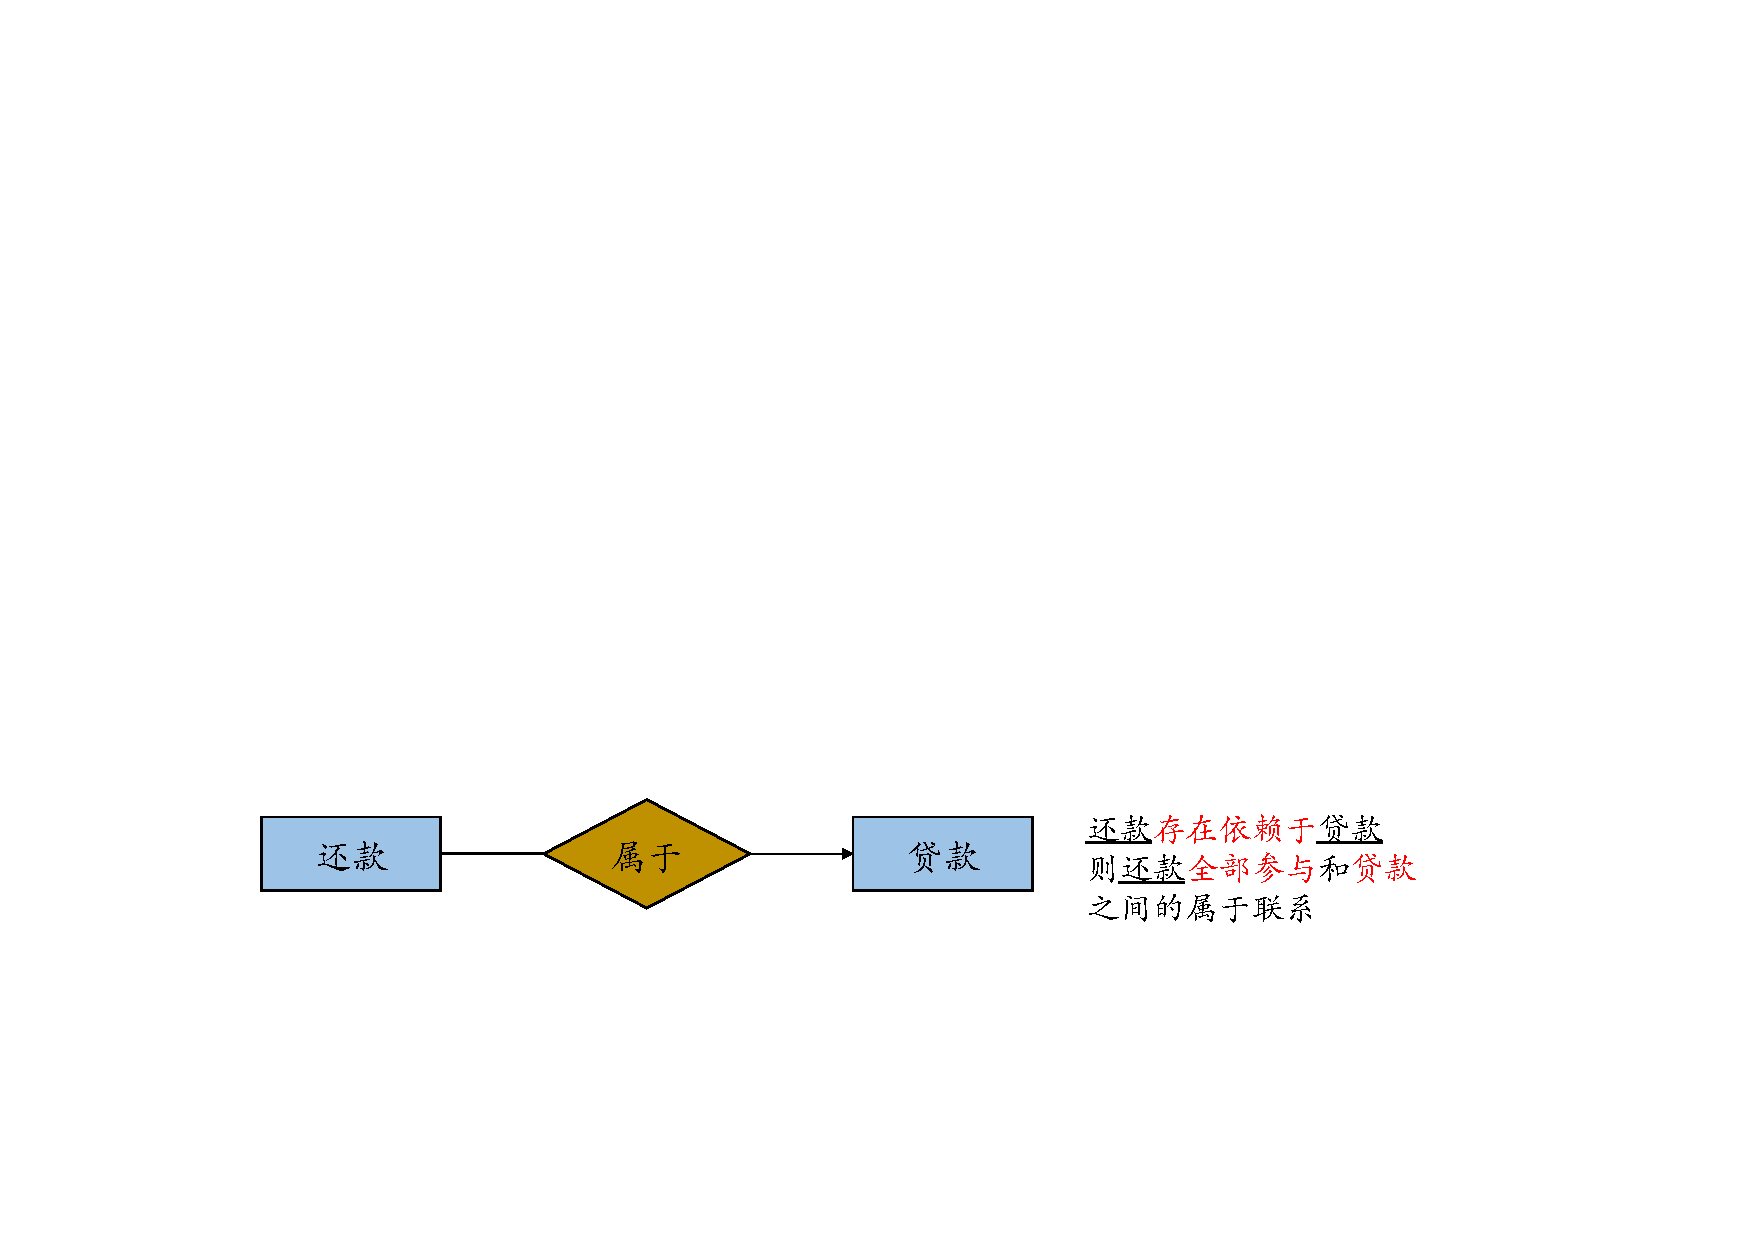
\includegraphics[width=.8\textwidth]{figure/存在依赖.pdf}
    \caption{存在依赖}
\end{figure}

复合实体. 一个 M:N 联系分解成两个 1:M. (了解即可.)

\section{扩展ER特性}

\begin{definition}[弱实体集 (weak entity set)]
    没有足够的属性以形成主码的实体集称为弱实体集.
\end{definition}

\begin{definition}[标识性联系 (identifying relationship)]
    弱实体集与其标识实体集相连的联系称为标识性联系 (identifying relationship). 其实就是弱实体集和强实体集的那一个联系.
\end{definition}

\begin{remark}
    弱实体集必然存在依赖于强实体集, 但是\textcolor{red}{存在依赖并不总会导致一个弱实体集}, 从属实体集可以有自己的主码.
\end{remark}

\begin{definition}[分辨符 (Discriminator)]
    弱实体集中用于区别依赖于某个特定强实体集的属性集合, 也称作部分码 (partial key).
\end{definition}

\textcolor{red}{!!!!!! 弱实体集的主码 = 强实体集的主码 + 弱实体集的分辨符}

\begin{figure}[H]
    \centering
    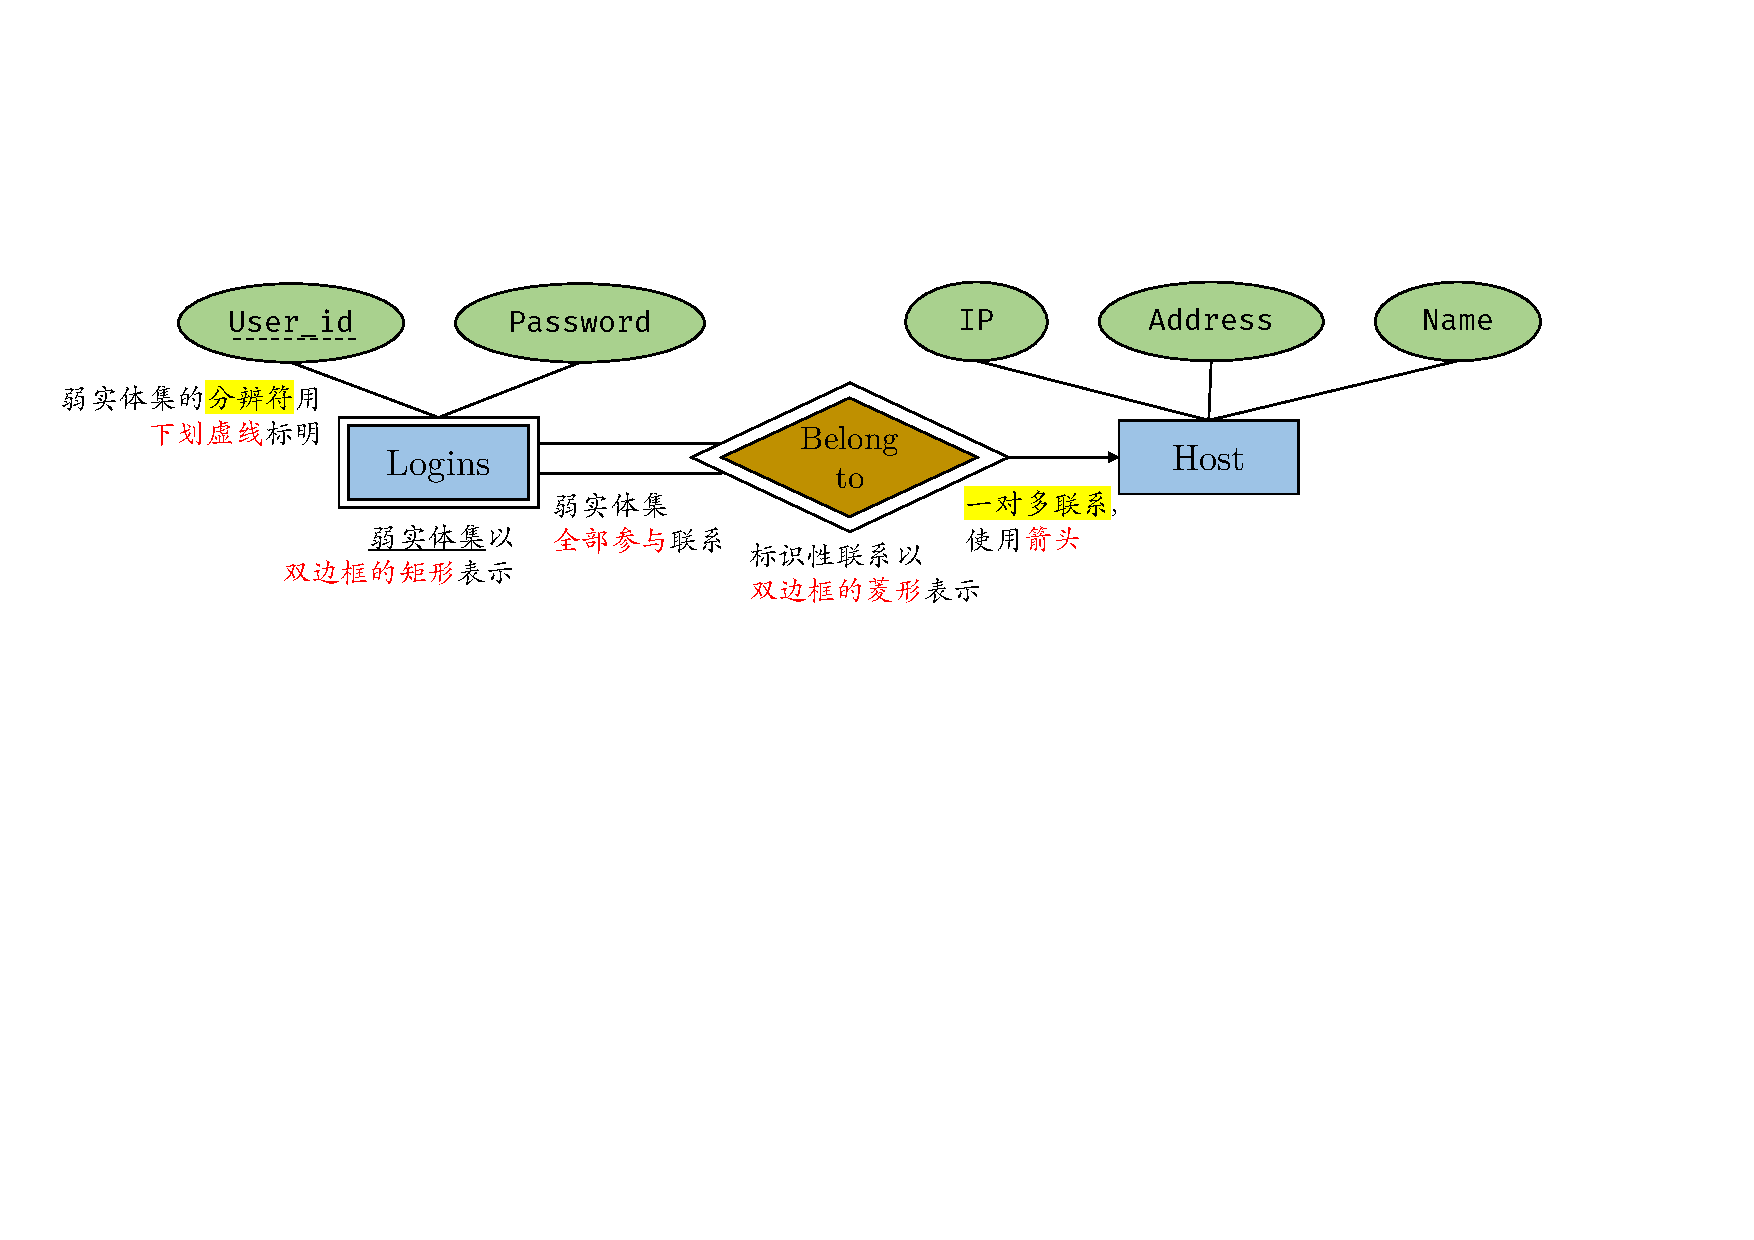
\includegraphics[width=\textwidth]{figure/弱实体集.pdf}
    \caption{弱实体集的ER表示}
\end{figure}

\begin{remark}
    何时引入弱实体集?
    \begin{itemize}
        \item 作为层次结构的一部分.
        \item 实体集的一些多值、复合属性可以抽取出来作为弱实体集.
        \item 如果弱实体集不但参与和强实体集之间的标识性联系, 
        而且参与和其它实体集的联系, 或者弱实体集本身含有很多属性, 则将其表述为弱实体集.
    \end{itemize}
\end{remark}

\begin{figure}[H]
    \centering
    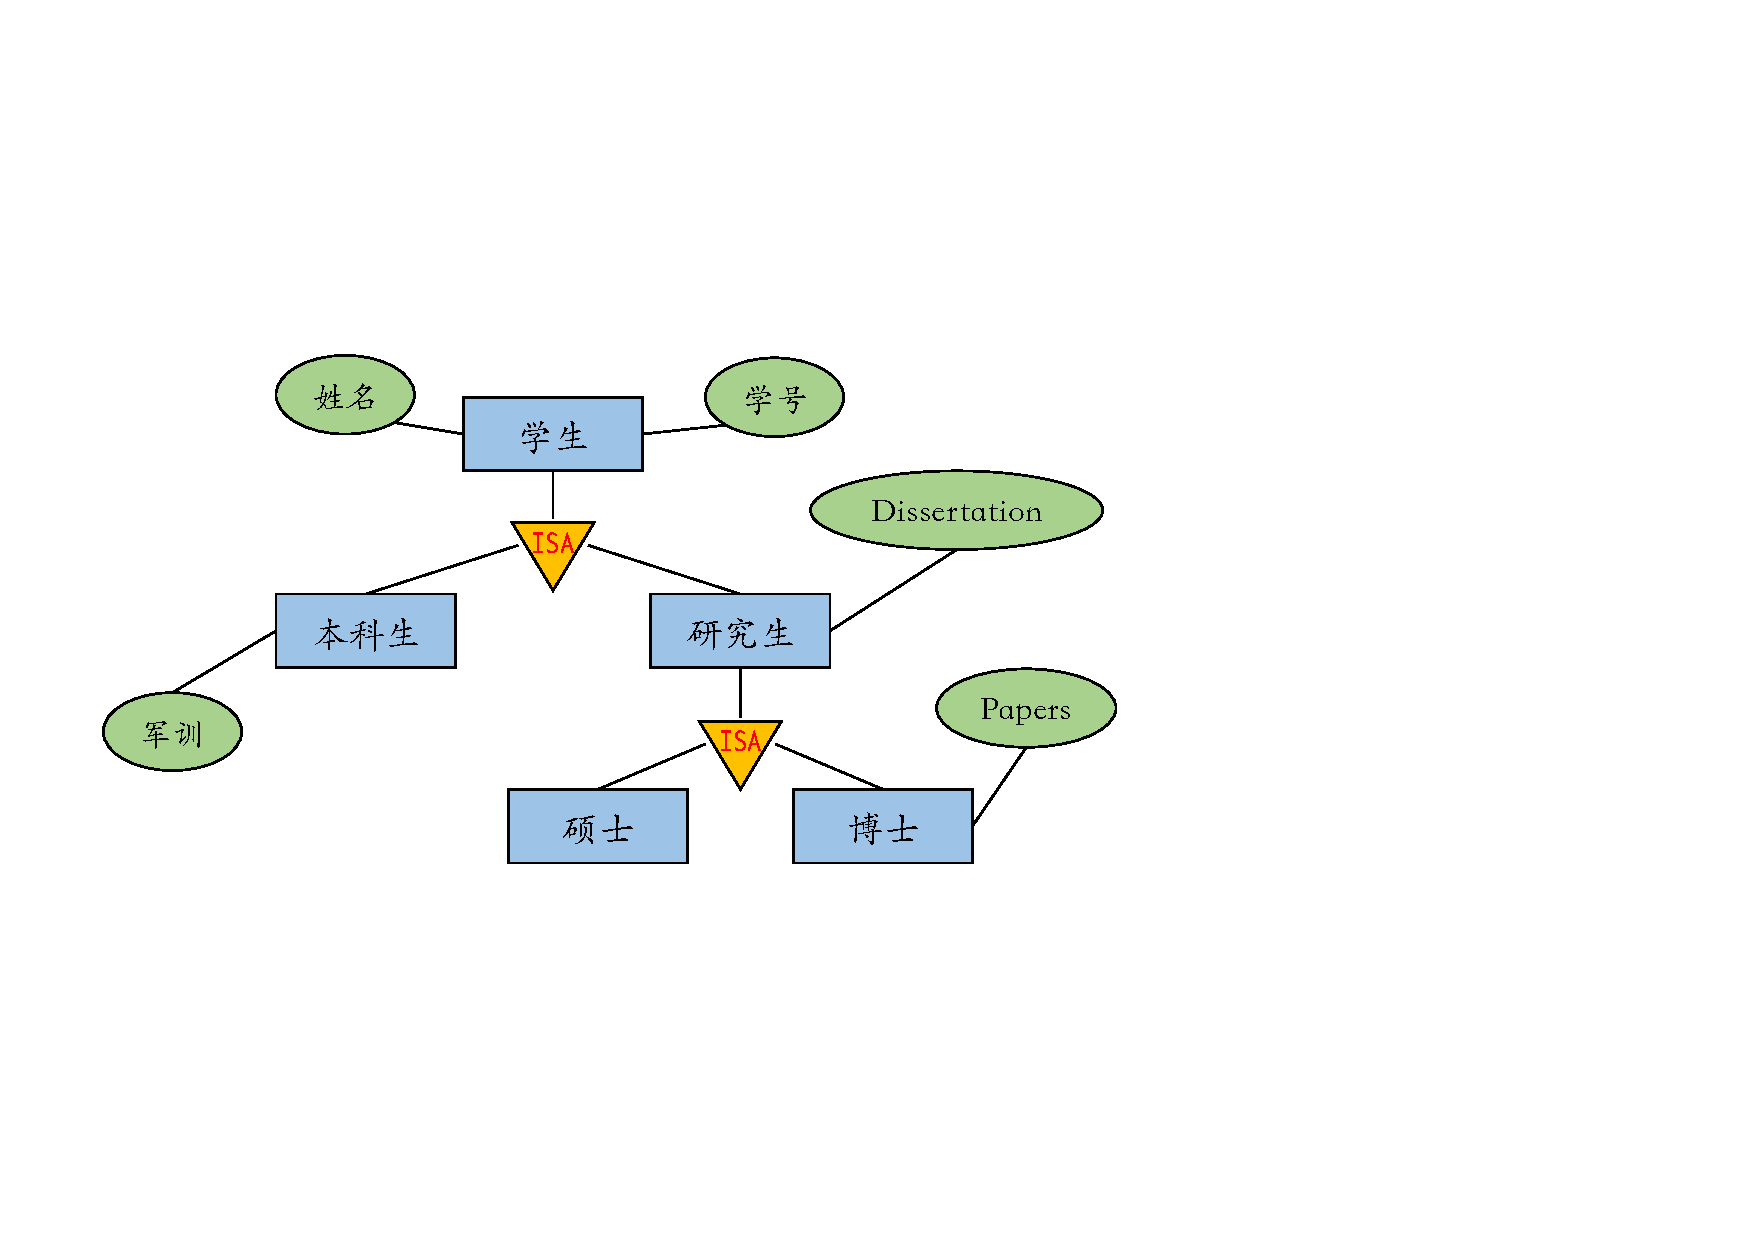
\includegraphics[width=.6\textwidth]{figure/特化.pdf}
    \caption{特化的ER表示}
\end{figure}

\begin{definition}[特化]
    实体集中某些子集具有区别于该实体集内其它实体的特性,可以根据这些差异特性对实体集进行分组,这一分组的过程称作特化. 标识为 ISA 的三角形. ISA = “is a”.
\end{definition}

\begin{definition}[概化]
    概化是高层实体集与一个或多个底层实体集的包含关系. 得到的 E-R 图和特化得到的 E-R 图是一样的, 只不过是自底向上.
\end{definition}

\begin{itemize}
    \item 层次结构(Hierarchy): 实体集作为低层实体集只能参与到一个ISA联系中.
    \item 格结构(Lattice): 低层实体集可以参与到多个ISA联系中.
\end{itemize}

\begin{figure}[H]
    \centering
    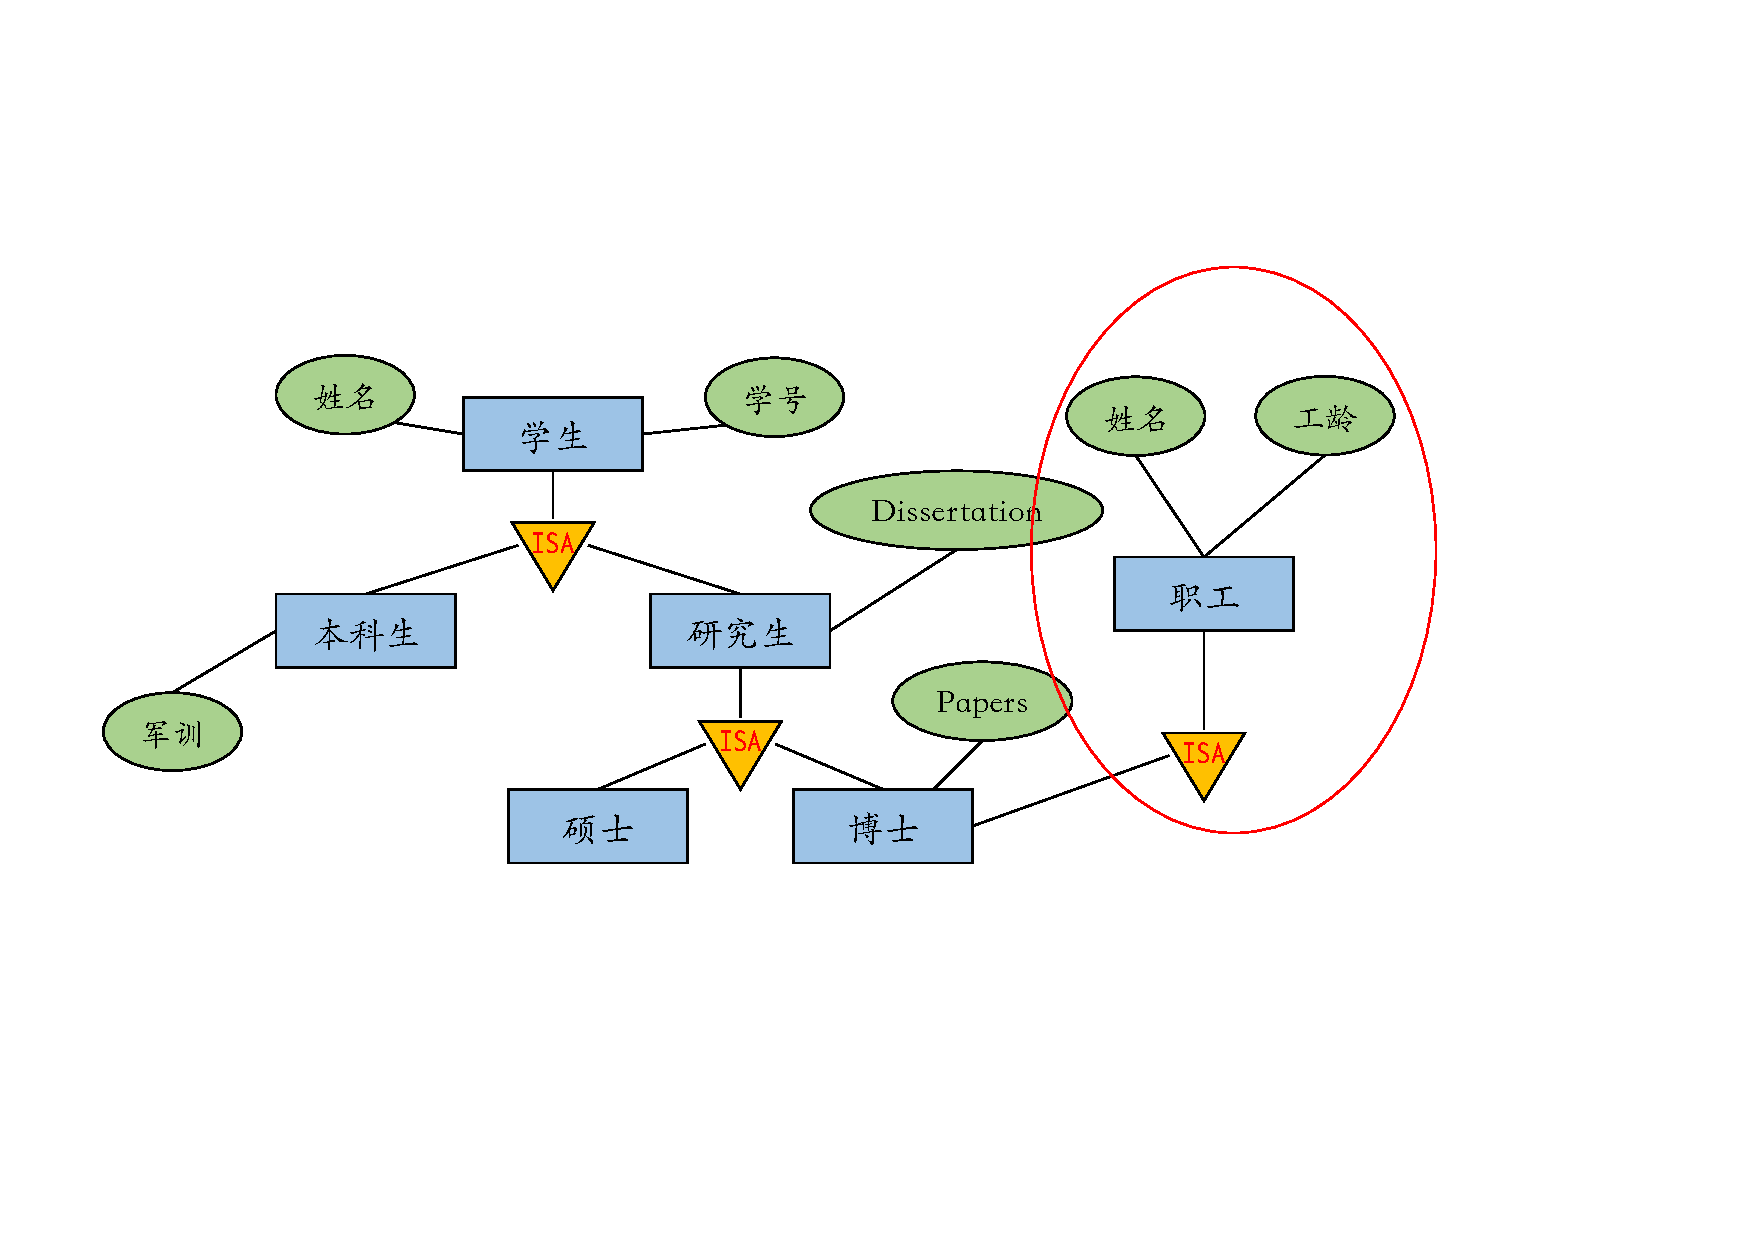
\includegraphics[width=.7\textwidth]{figure/格结构.pdf}
    \caption{格结构}
\end{figure}

概化中的成员身份:
\begin{itemize}
    \item 不相交的 (Disjoint): 一个实体至多属于一个低层实体集. e.g., 学生只能参加一个项目组, 学生就是不相交成员身份.
    \item 有重叠的 (Overlapping): 同一实体可同时属于同一概化的多个低层实体集. e.g., 老师可以参加多个项目组, 老师就是有重叠成员身份.
\end{itemize}

概化中的全部性约束: 确定高层实体集中的一个实体是否\textbf{必须}属于至少一个低层实体集.
\begin{itemize}
    \item 全部的 (Total): 每个高层实体必须属于一个低层实体集. e.g., 学生必须属于本科生或者研究生其中一种.
    \item 部分的 (Partial): 允许一些高层实体不属于任何低层实体集. e.g., 学生可以不属于任何的项目组.
\end{itemize}

\begin{definition}[聚集]
    两个先后动作的序列.
\end{definition}

\begin{figure}[H]
    \centering
    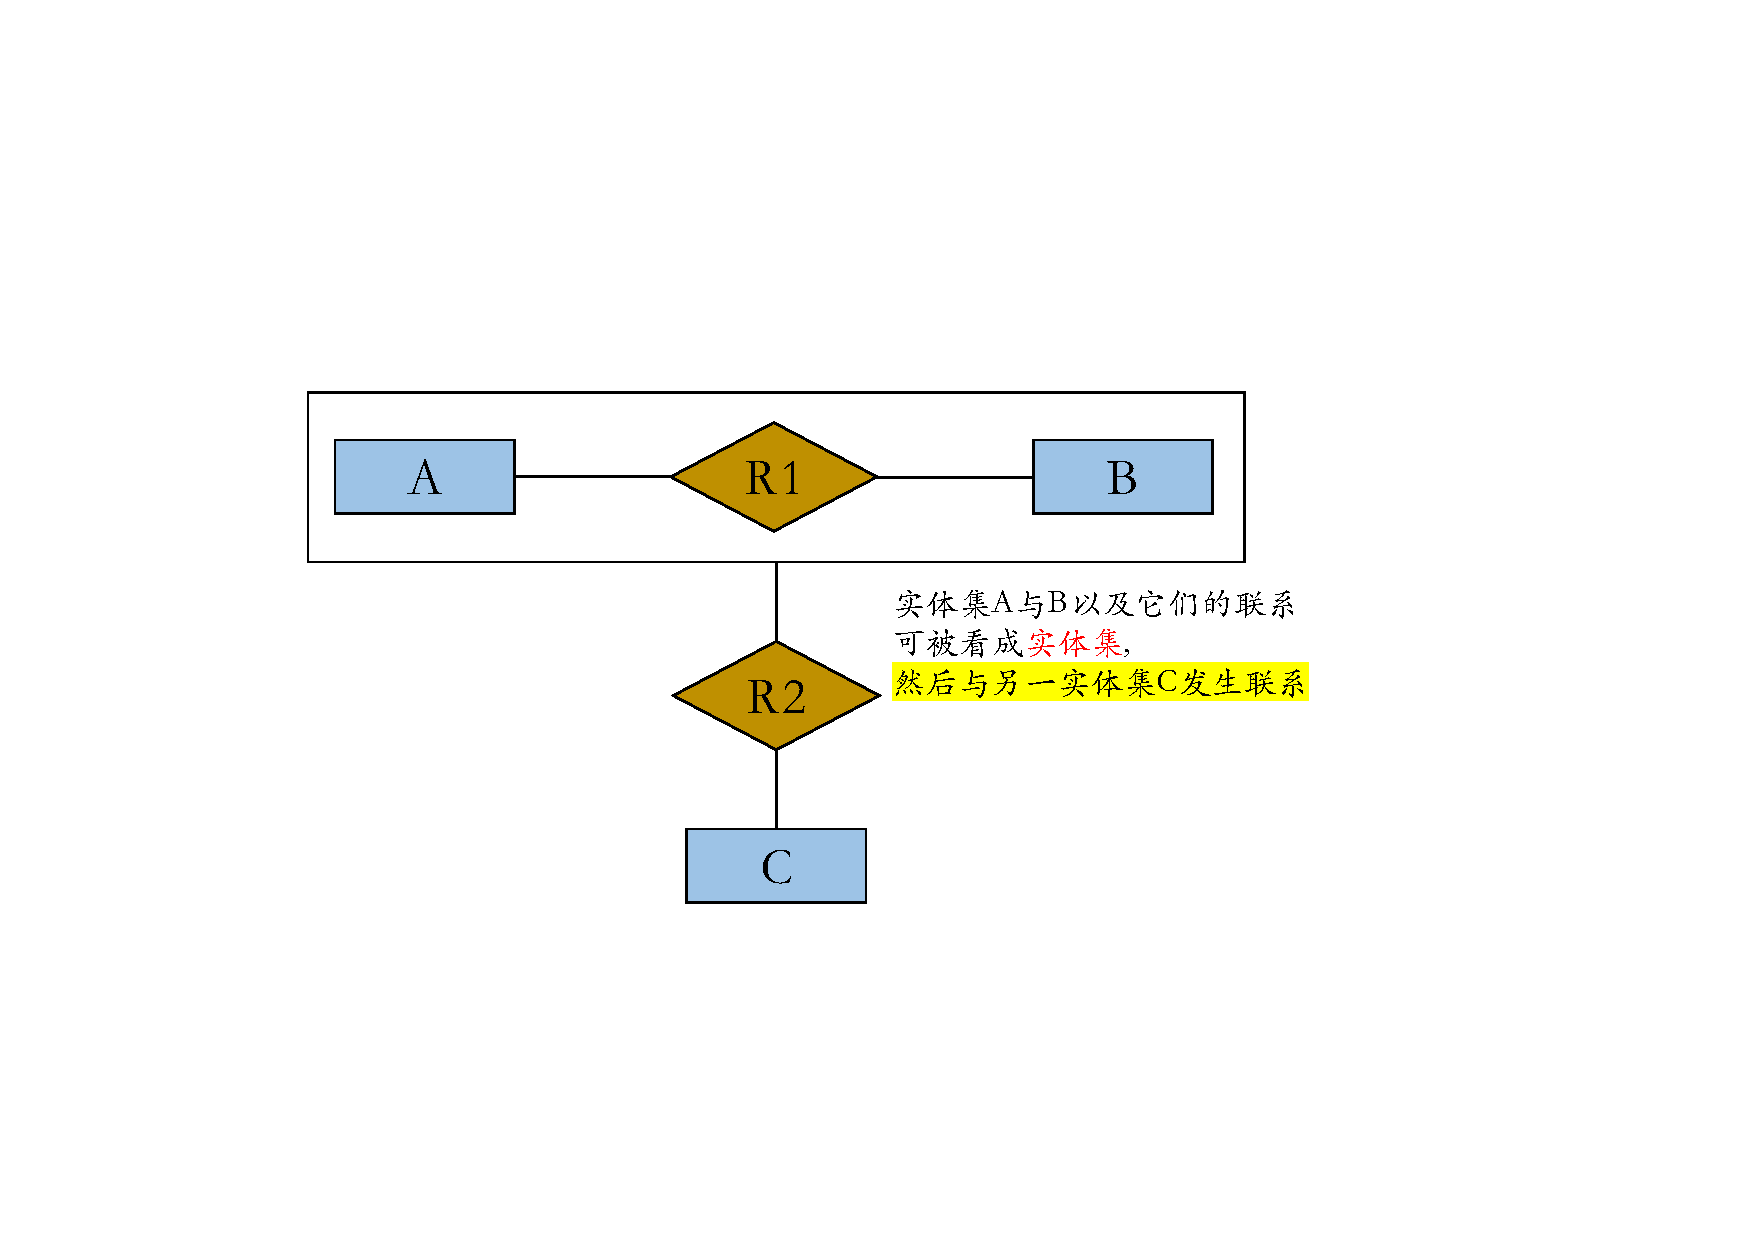
\includegraphics[width=.5\textwidth]{figure/聚集.pdf}
    \caption{聚集的ER表示}
\end{figure}


\begin{example}
    能否把多元联系转换为若干个二元联系?
\end{example}

新构建一个\textcolor{red}{标识实体集}$E$, 构造三个新联系集$R_A, R_B, R_C$, 对于每个$(a_i,b_i,c_i)\in R$, 在$E$中创建一个$e_i$, 然后在$R_A, R_B, R_C$中分别加入联系$(e_i,a_i),(e_i,b_i),(e_i,c_i)$.

这样的转换并无实际意义.

\begin{figure}[H]
    \centering
    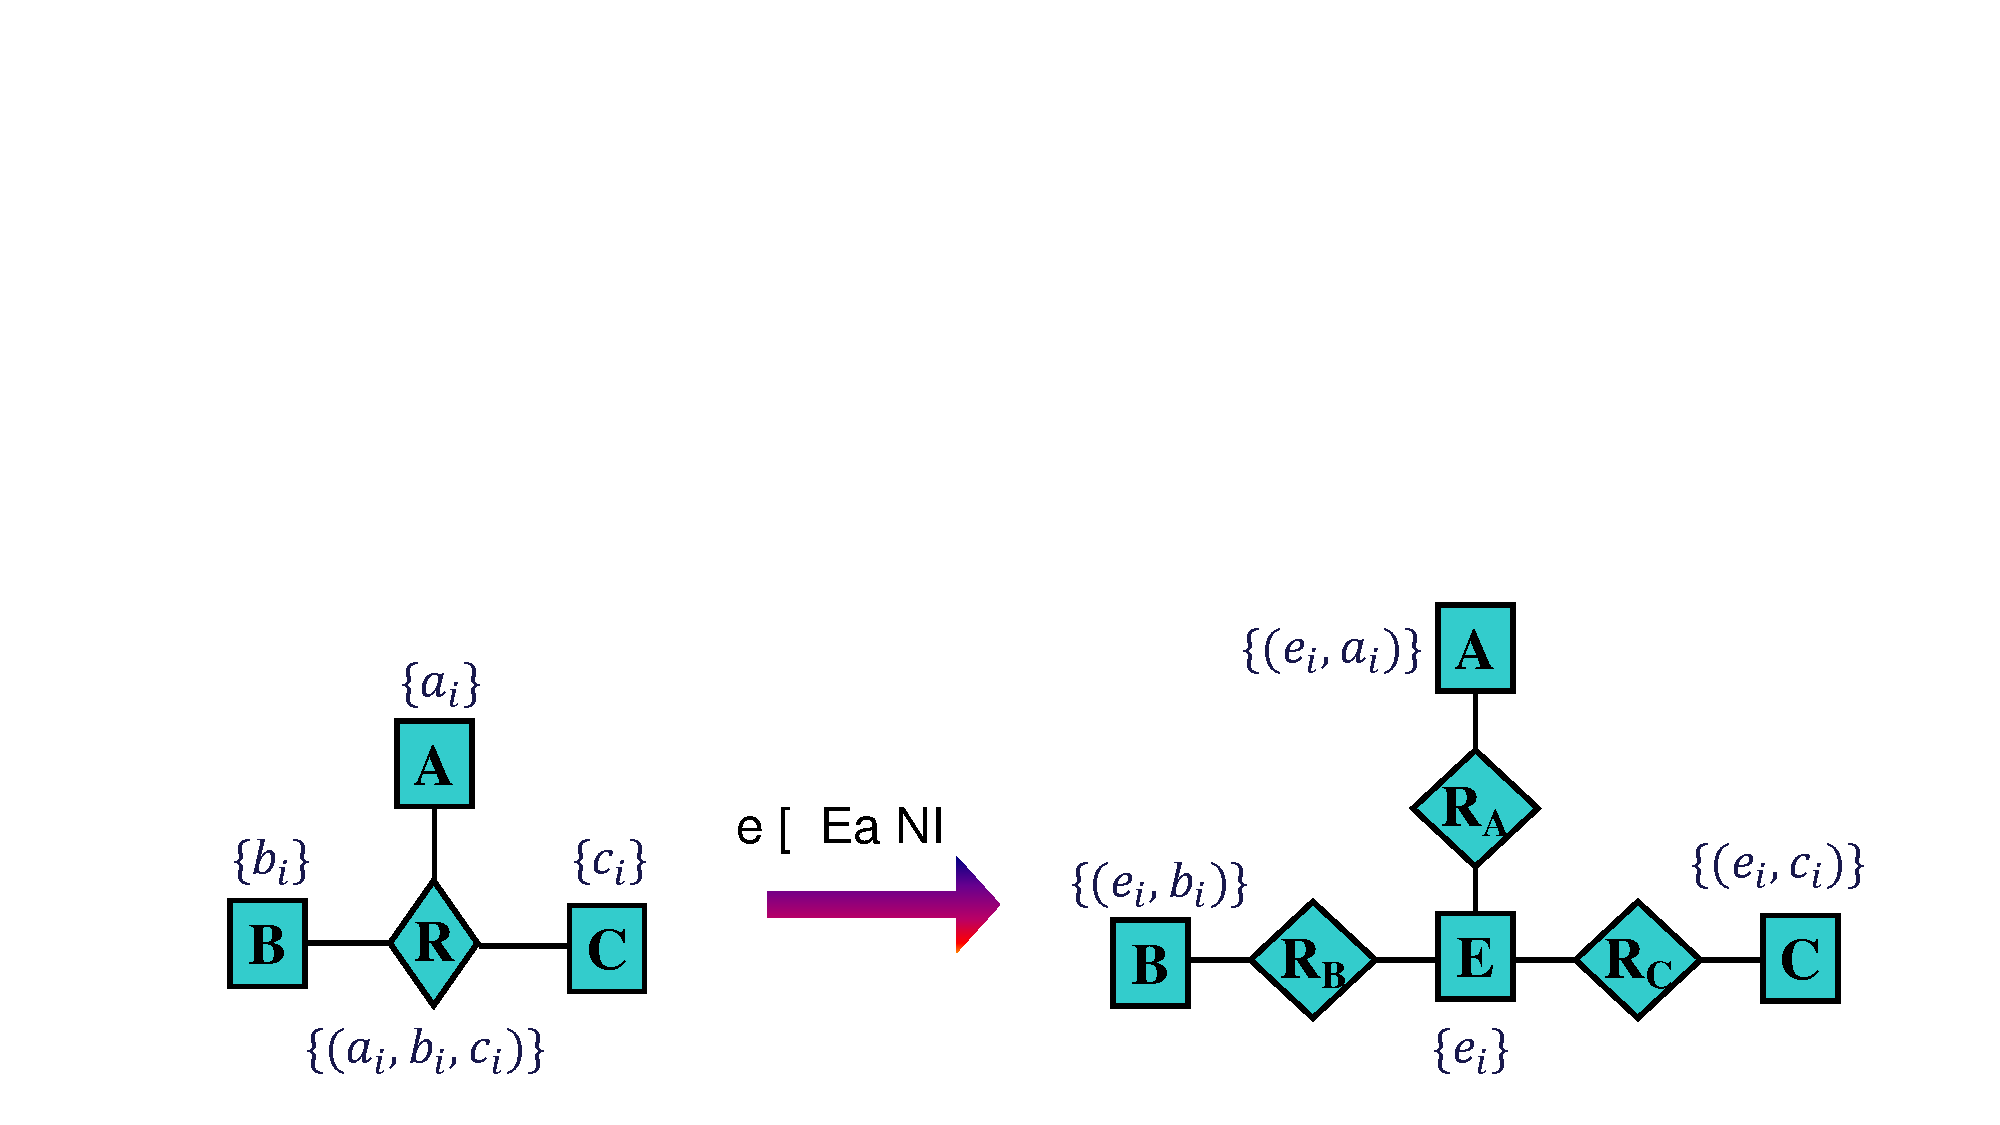
\includegraphics[width=.8\textwidth]{figure/无意义转换.pdf}
    \caption{无意义的转换}
\end{figure}

\section{概念数据库设计过程}

\begin{itemize}
    \item 局部ER模式设计.
    \item 全局ER模式设计.
    \item 全局ER模式优化.
\end{itemize}

\section{ER模型向关系模式的转换}

\begin{enumerate}
    \item 实体 $\to$ 关系.
    \item 属性 $\to$ 关系的属性.
    \begin{enumerate}
        \item 复合属性定义为视图, 或者由应用定义, 这里摊平即可.
        \item 多值属性 $\to$ 新的关系 + (取值+所在实体的码)
    \end{enumerate}
    \item 一对多联系 $\to$ 将单方参与实体的码作为多方参与实体的属性.
    \item 多对多联系 $\to$ 将联系定义为新的关系, 属性为参与双方的码.
    \item 一对一联系 $\to$ 若联系双方均部分参与, 则将联系定义为一个新的关系, 属性为参与双方的码. 全部参与同一对多.
    \item 弱实体集 $\to$ 弱实体集所对应的关系的码由弱实体集本身的分辨符再加上所依赖的强实体集的码.
    \item 概化 $\to$ 高层实体集和低层实体集分别转为表, 低层实体集所对应的关系包括高层实体集的码.
    \item 聚集 $\to$ 实体集A与B及其联系R被抽象成实体集C, C与另一实体集D构成联系S, 则S的码由C和D的码构成.
\end{enumerate}

\section{关系模式向ER的转换}

!识别关系间的重合属性.

\begin{itemize}
    \item 出现$Tb(\underline{a_3, a_5},a_7)$, 这种情况时, 且$a_3, a_5$是别的关系的码, 则建模为关系
    \item 出现了了$Tb1(\underline{a_1},a_2,a_3), Tb2(\underline{a_3}, a_4)$这样的重合时, 之间是一对多的关系
\end{itemize}

\begin{figure}[H]
    \centering
    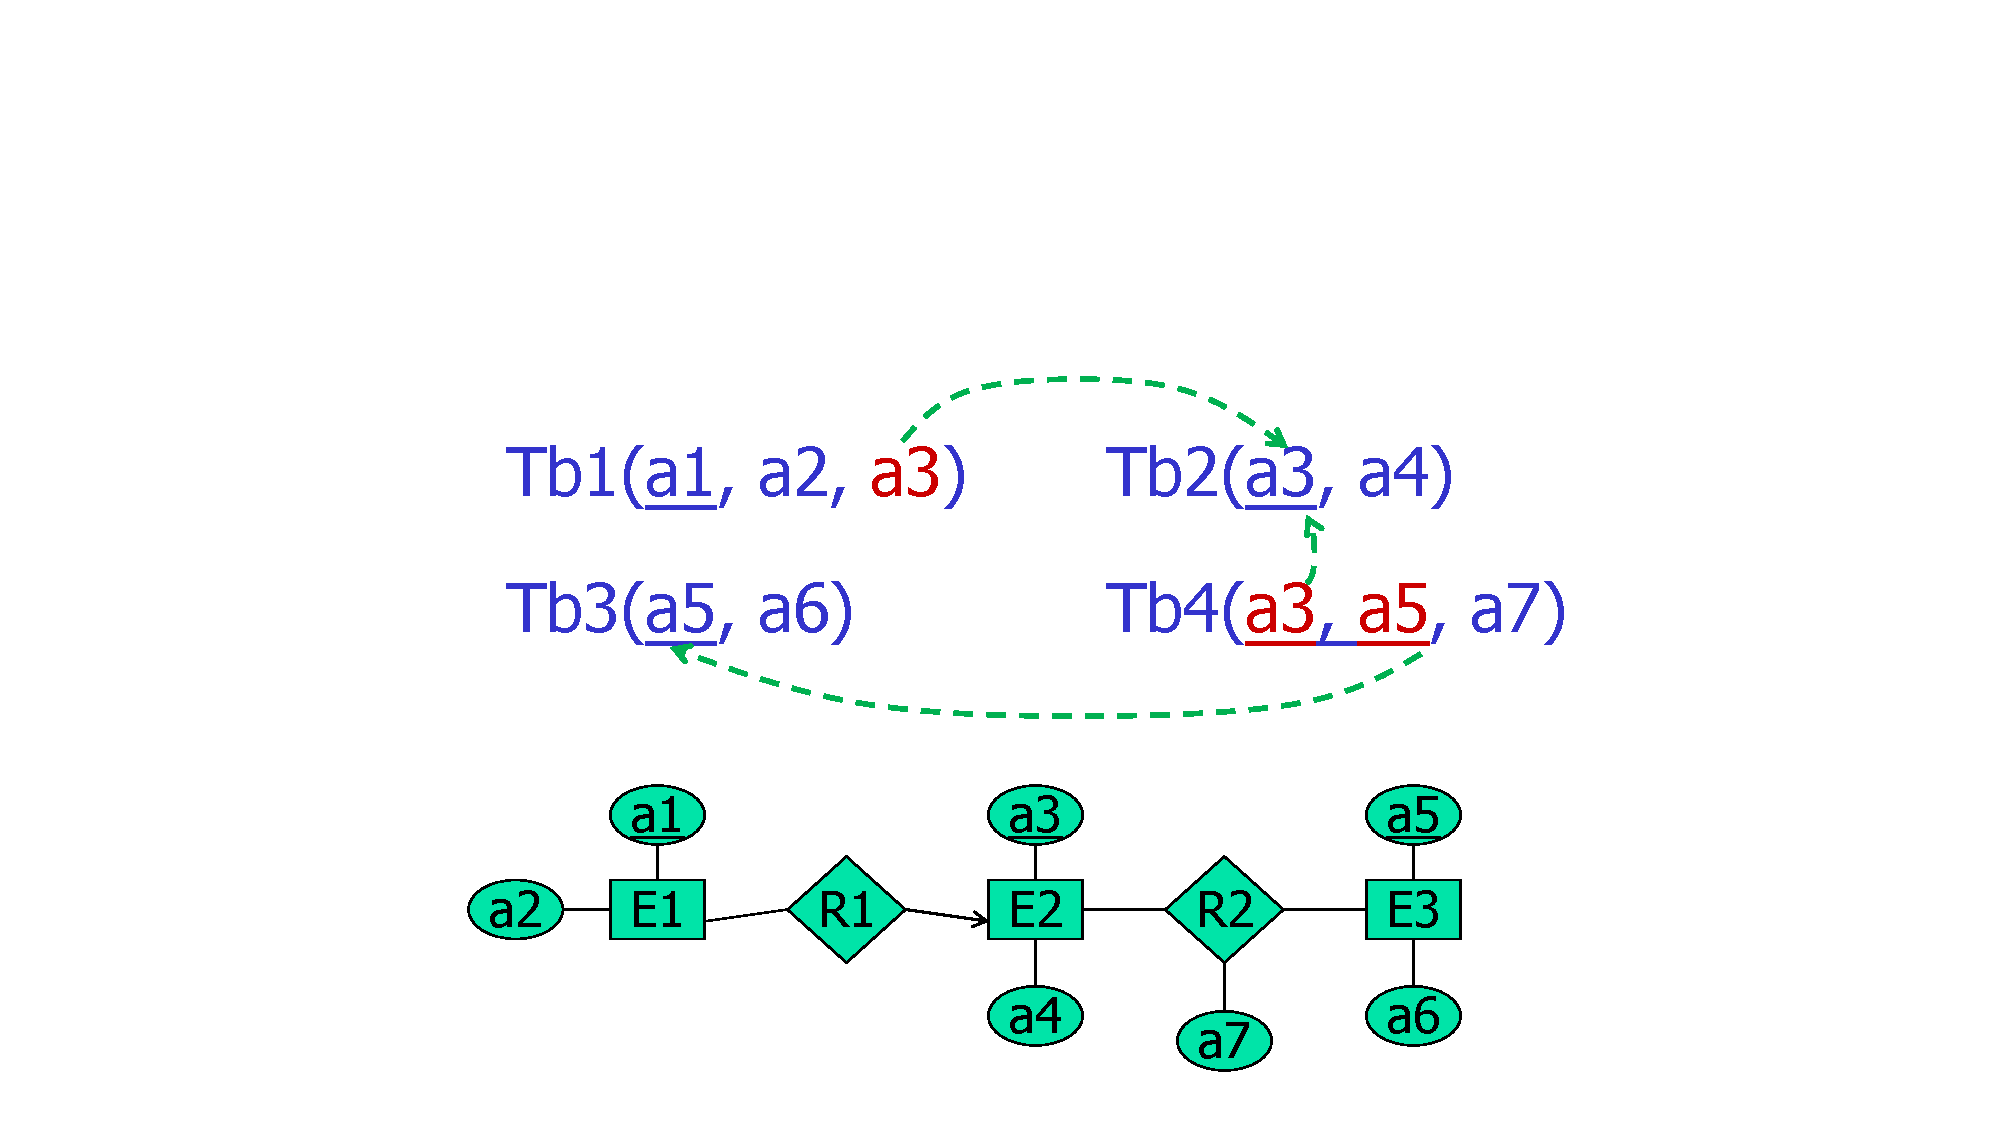
\includegraphics[width=.5\textwidth]{figure/逆向转换.pdf}
    \caption{逆向转换}
\end{figure}

\begin{problemset}
    \item 分别列举聚集、弱实体、细化/泛化的实用例子, 记得不要同讲义上的相同. 说明在此时采用这些扩展表示方法的优点.
    \item 已知有如下关系模式: 
  \begin{eqnarray*}
    R_1 \left( \text{} \underline{a_1}, a_2, a_3 \right), & R_2 \left(
    \underline{a_3}, a_4, a_1 \right), & R_3 \left( \underline{a_5}, a_6
    \right),\\
    R_4 \left( \underline{a_3, a_5}, a_7 \right), & R_5 \left( \underline{a_1,
    a_3, a_5}, a_8 \right) & 
  \end{eqnarray*}
  其中带下划线的属性标识为所在关系模式的主码, 关系模式之间重合的属性是主外码关系, 体现了实体之间的联系.
  
  试画出相应的E-R图, 使得可以从该E-R图推导出上述关系模式.
  \item 下面是一张NBA球员转会的汇总表格, 基于这些表格中的数据, 请画出合适的ER图.
  \begin{table}[H]
\centering
\begin{tabular}{|c|c|c|c|c|c|c|c|}
\hline
交易ID & 转出球队 & 转出球队薪酬总额 & 转入球队 & 转入球队薪酬总额 & 交易球员 & 球员工资 & 交易时间 \\
\hline
T001 & 湖人 & 7500 & 骑士 & 8500 & 科比 & 3000 & 2016.05.07 \\
\hline
T001 & 骑士 & 8500 & 湖人 & 7500 & 勒布朗 & 2300 & 2016.05.07 \\
\hline
T001 & 勇士 & 7000 & 骑士 & 8500 & 库里 & 1500 & 2016.05.07 \\
\hline
T001 & 湖人 & 7500 & 勇士 & 7000 & 费舍尔 & 700 & 2016.05.07 \\
\hline
T001 & 骑士 & 8500 & 勇士 & 7000 & 欧文 & 800 & 2016.05.07 \\
\hline
T002 & 雷霆 & 8000 & 快船 & 8300 & 韦斯布鲁克 & 1200 & 2016.07.07 \\
\hline
T002 & 快船 & 8300 & 雷霆 & 8000 & 保罗 & 1200 & 2016.07.07 \\
\hline
\end{tabular}
\caption{球员交易记录表}
\label{tab:player_transactions}
\end{table}
    \item 假定以下是存储微信内容的数据库相关表, 请根据这些表画出微信的ER图.
    \begin{itemize}
    \item 信友({\underline{信友ID}}, 信友名, 昵称, 所在区域, 手机号)
    \item 通讯录({\underline{信友1 ID,信友2 ID}},认识方式,认识时间)
    \item 群({\underline{群ID}},群名称,群类型,创建时间,群主ID)
    \item 群成员({\underline{群ID,信友ID}},加入时间,引介人ID,信友群内昵称)
    \item 帖子({\underline{帖子ID}},发帖信友ID,所属群ID,帖子内容,发帖时间)
    \item 短信({\underline{短信ID}},发送信友ID,接受信友ID,短信时间,短信内容)
  \end{itemize}
  \item 对于一个论文评审数据库,记录有如下信息: 
  \begin{itemize}
    \item 论文有{\underline{论文ID}}、标题、摘要、所属主题(一个)、作者(多位)、通讯作者(一位)
    \item 作者有{\underline{作者ID}}、姓名、投稿论文(多篇)
    \item 审稿人有{\underline{审稿人ID}}、email、所关心的主题(多个)
    \item 主题有{\underline{主题ID}}、名称、主持人(由一位审稿人主持)
    \item 每篇论文分配给4位审稿人,从可读性、创新性、相关性打分(1\~{}10分)
    \item 每位审稿人生成书面意见反馈给通讯作者
  \end{itemize}
  请根据以上描述,画出其ER图.
  \item 考察航班、航线、机场、机组、飞机、飞行员之间的业务关系,先罗列出来,尽可能地与实际情况相符,然后再画出相应的ER图.
  
  另外,MySQL自带了一个airport数据库,这个链接提供了相应的文档描述,\url{https://downloads.mysql.com/docs/airportdb-en.a4.pdf}.同学们也可以基于它来直接完成概念建模.
  
  airportdb的表结构如下图所示(可以询问大模型如何将下面的表关联图转换为ER模型):
  \begin{figure}[H]
      \centering
      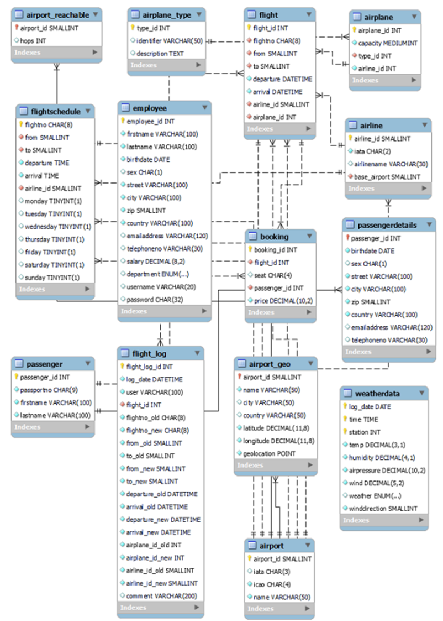
\includegraphics[width=.5\textwidth]{figure/第2章-7.pdf}
      \caption{airportdb的表结构}
  \end{figure}
  \item 请向大模型提问你感兴趣的业务系统,请它返回响应的数据库设计,然后再借助大模型把表格转为ER模型.
  \begin{itemize}
    \item 请设计一个数据库表结构能支持知乎网站的典型应用
    \item 请设计一个数据库表结构能支持电子商务网站的典型应用
  \end{itemize}
\end{problemset}

